%%%%%%%%%%%%%%% fittings
\section{The comparisons of sinusoidal friction model with experimental force-displacement curves for 22  simply-supported tests with sawtooth pattern}
\label{sec:comparison}


\newpage
\begin{figure}[H]
\subfigure{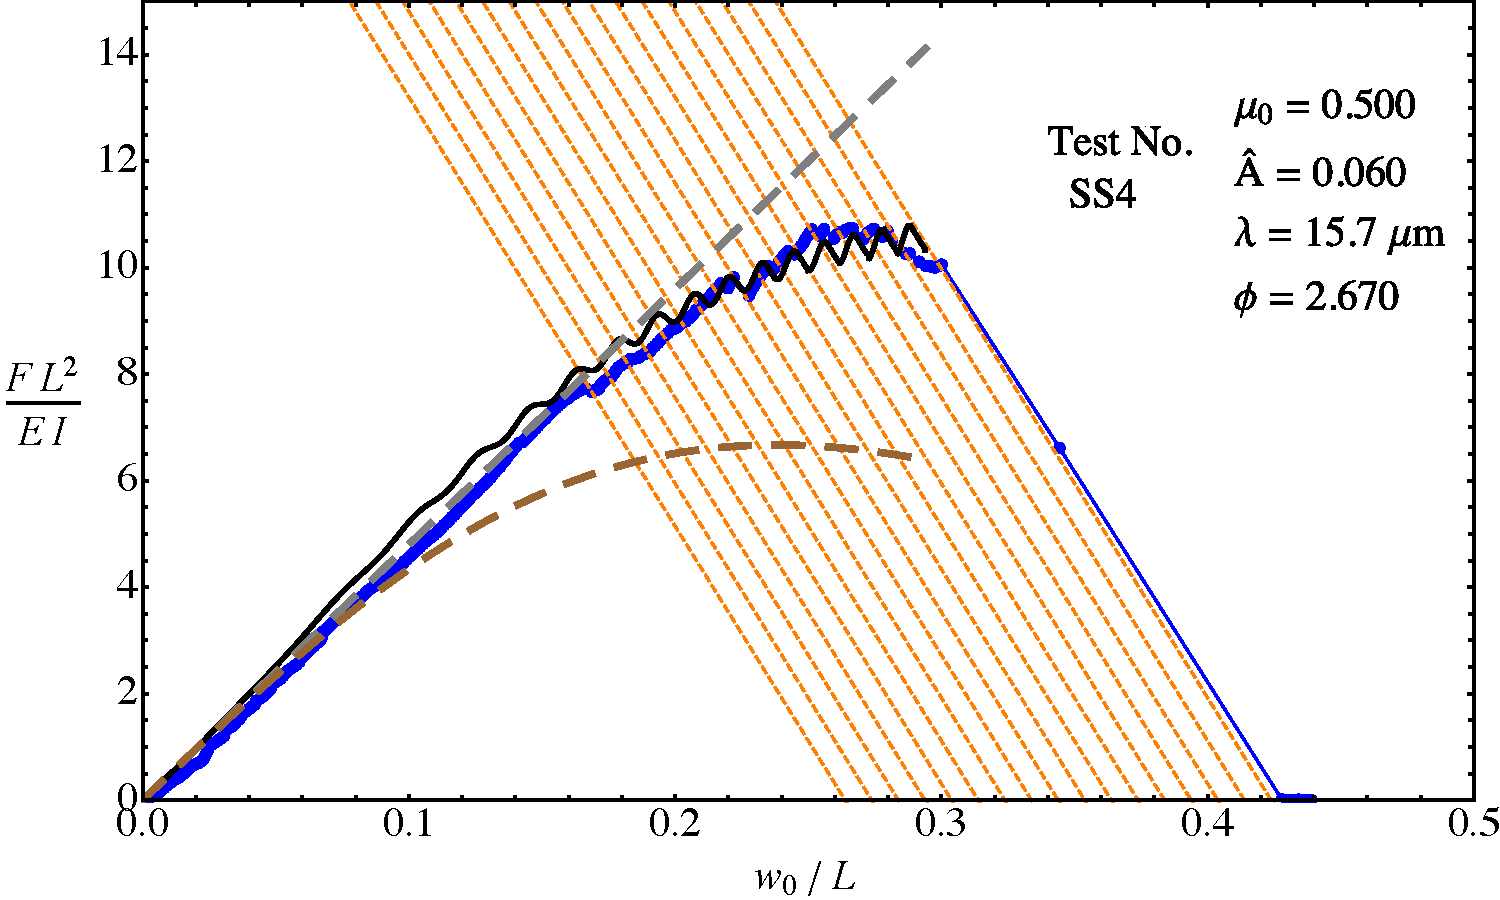
\includegraphics[width = .5\linewidth]{Figures/ComparisonThreeModels/Fitting01.pdf}}
\subfigure{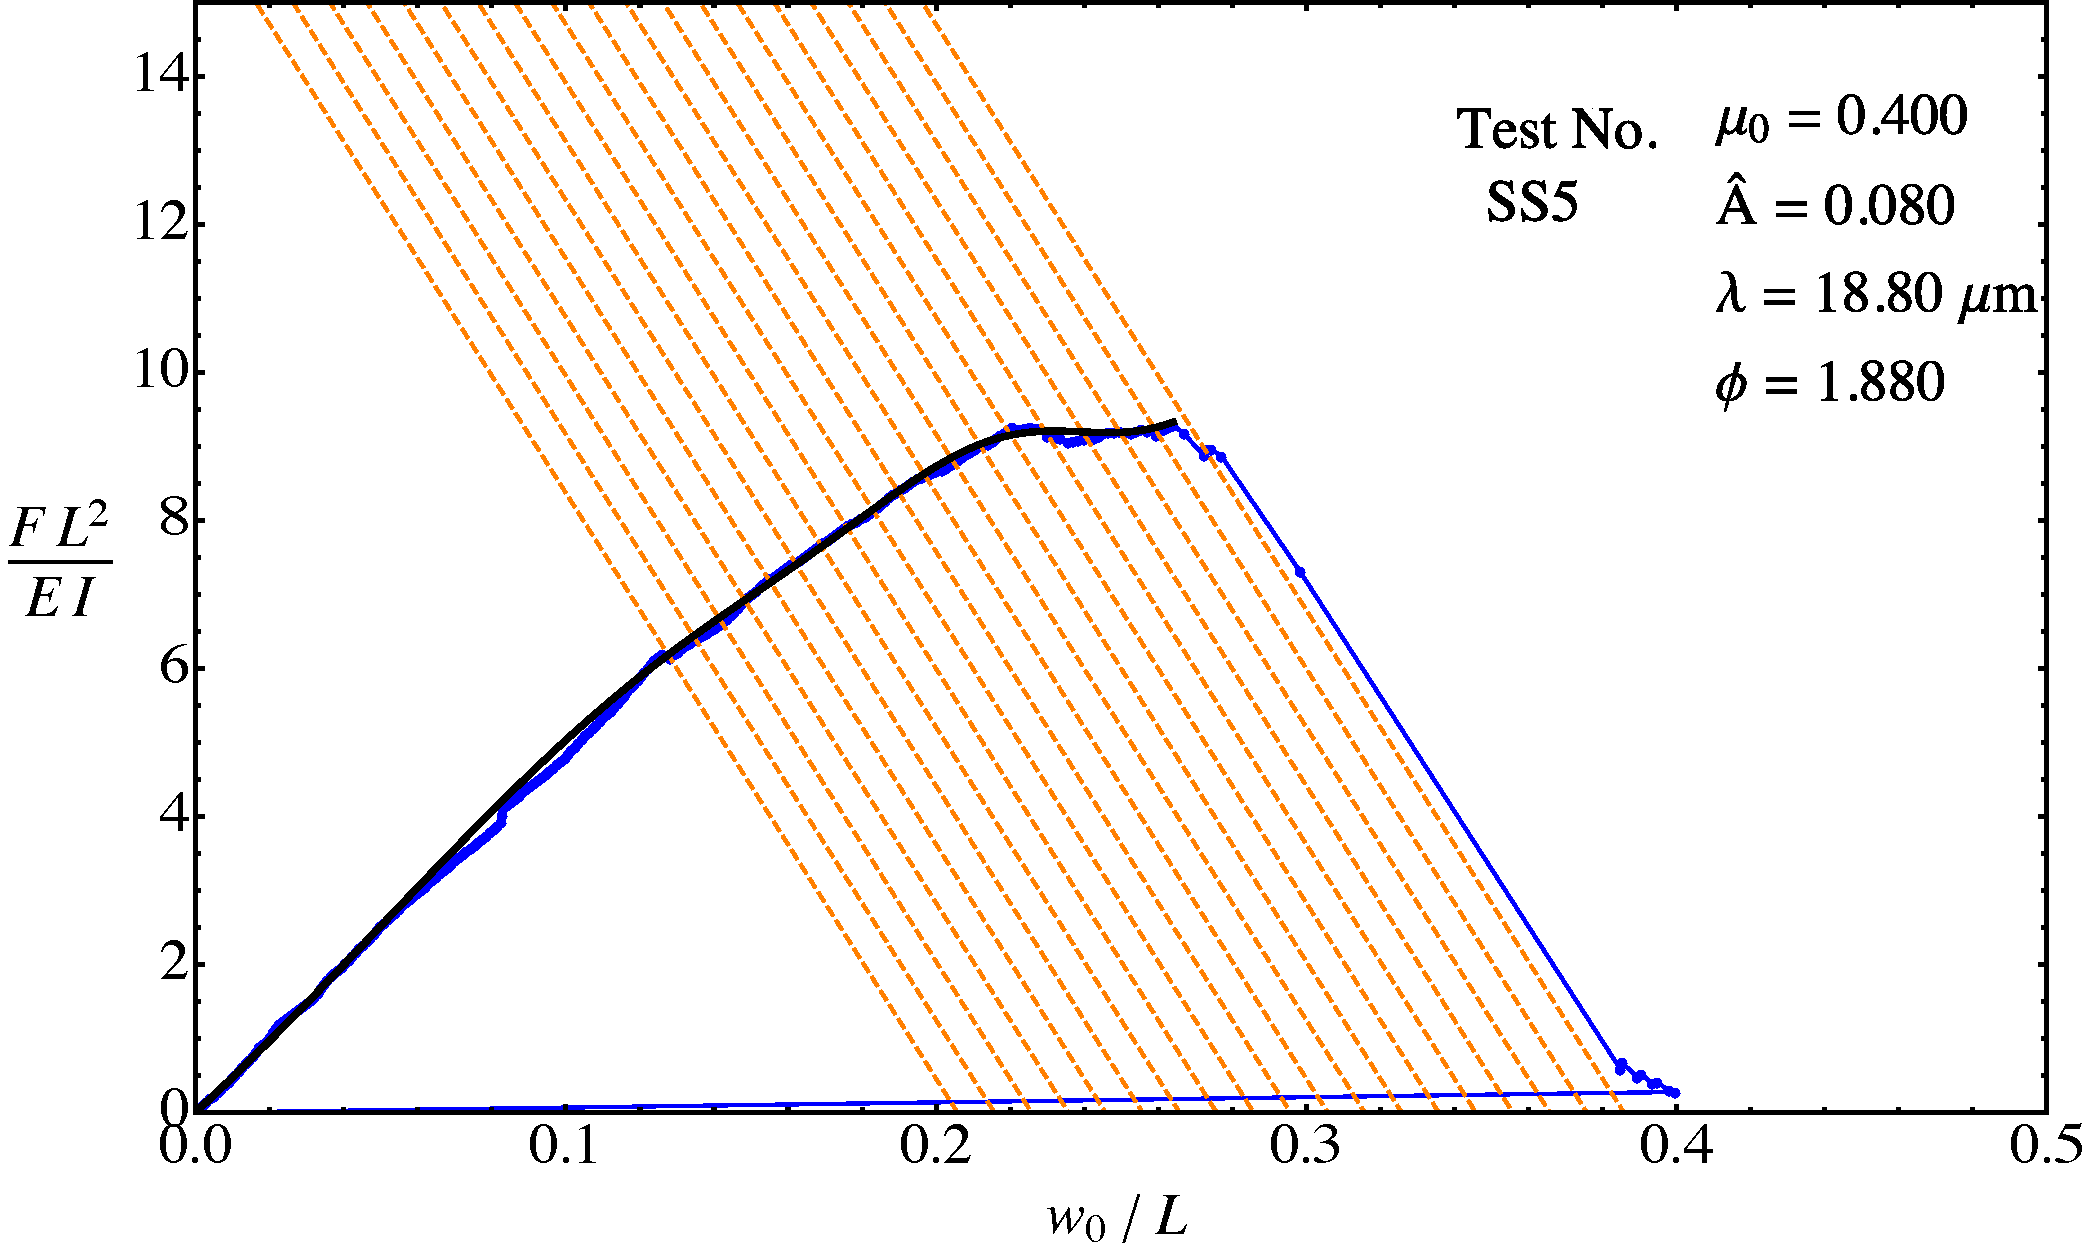
\includegraphics[width = .5\linewidth]{Figures/ComparisonThreeModels/Fitting02.pdf}}
\subfigure{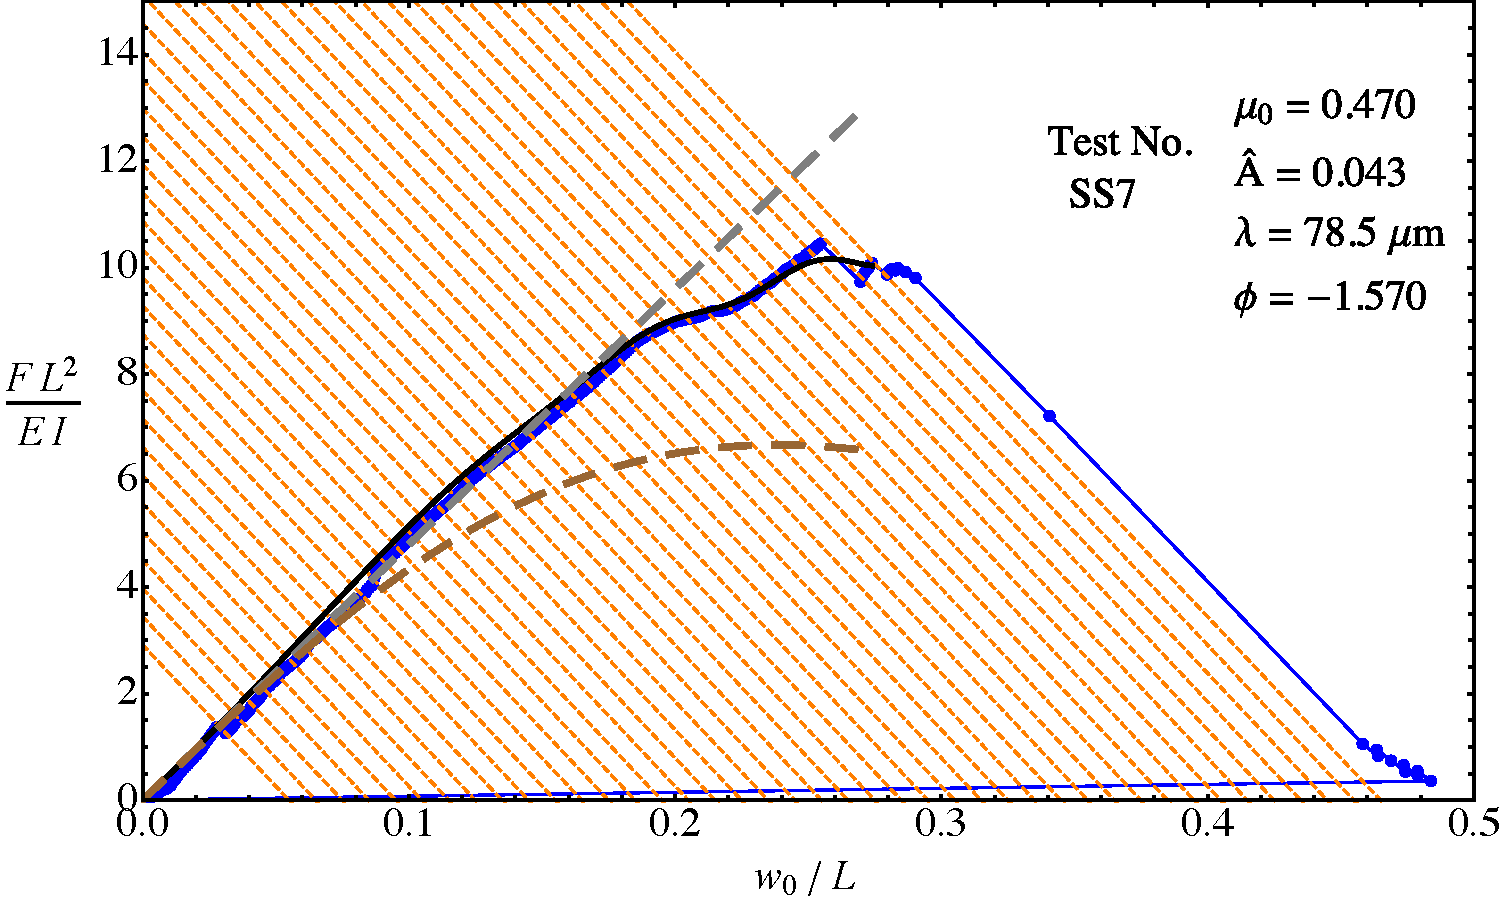
\includegraphics[width = .5\linewidth]{Figures/ComparisonThreeModels/Fitting03.pdf}}
\subfigure{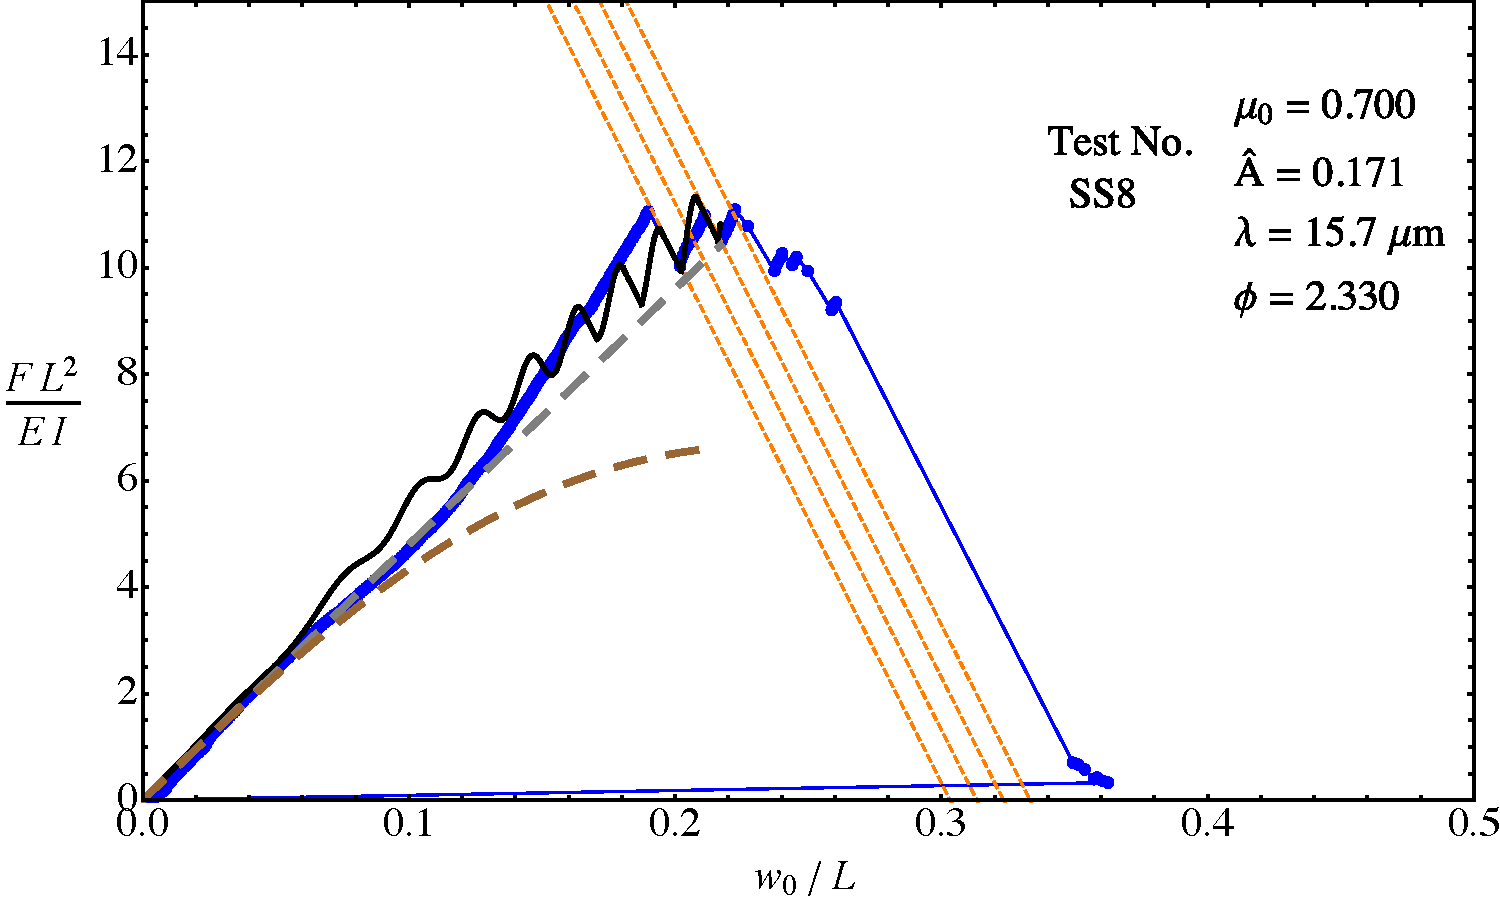
\includegraphics[width = .5\linewidth]{Figures/ComparisonThreeModels/Fitting04.pdf}}
\subfigure{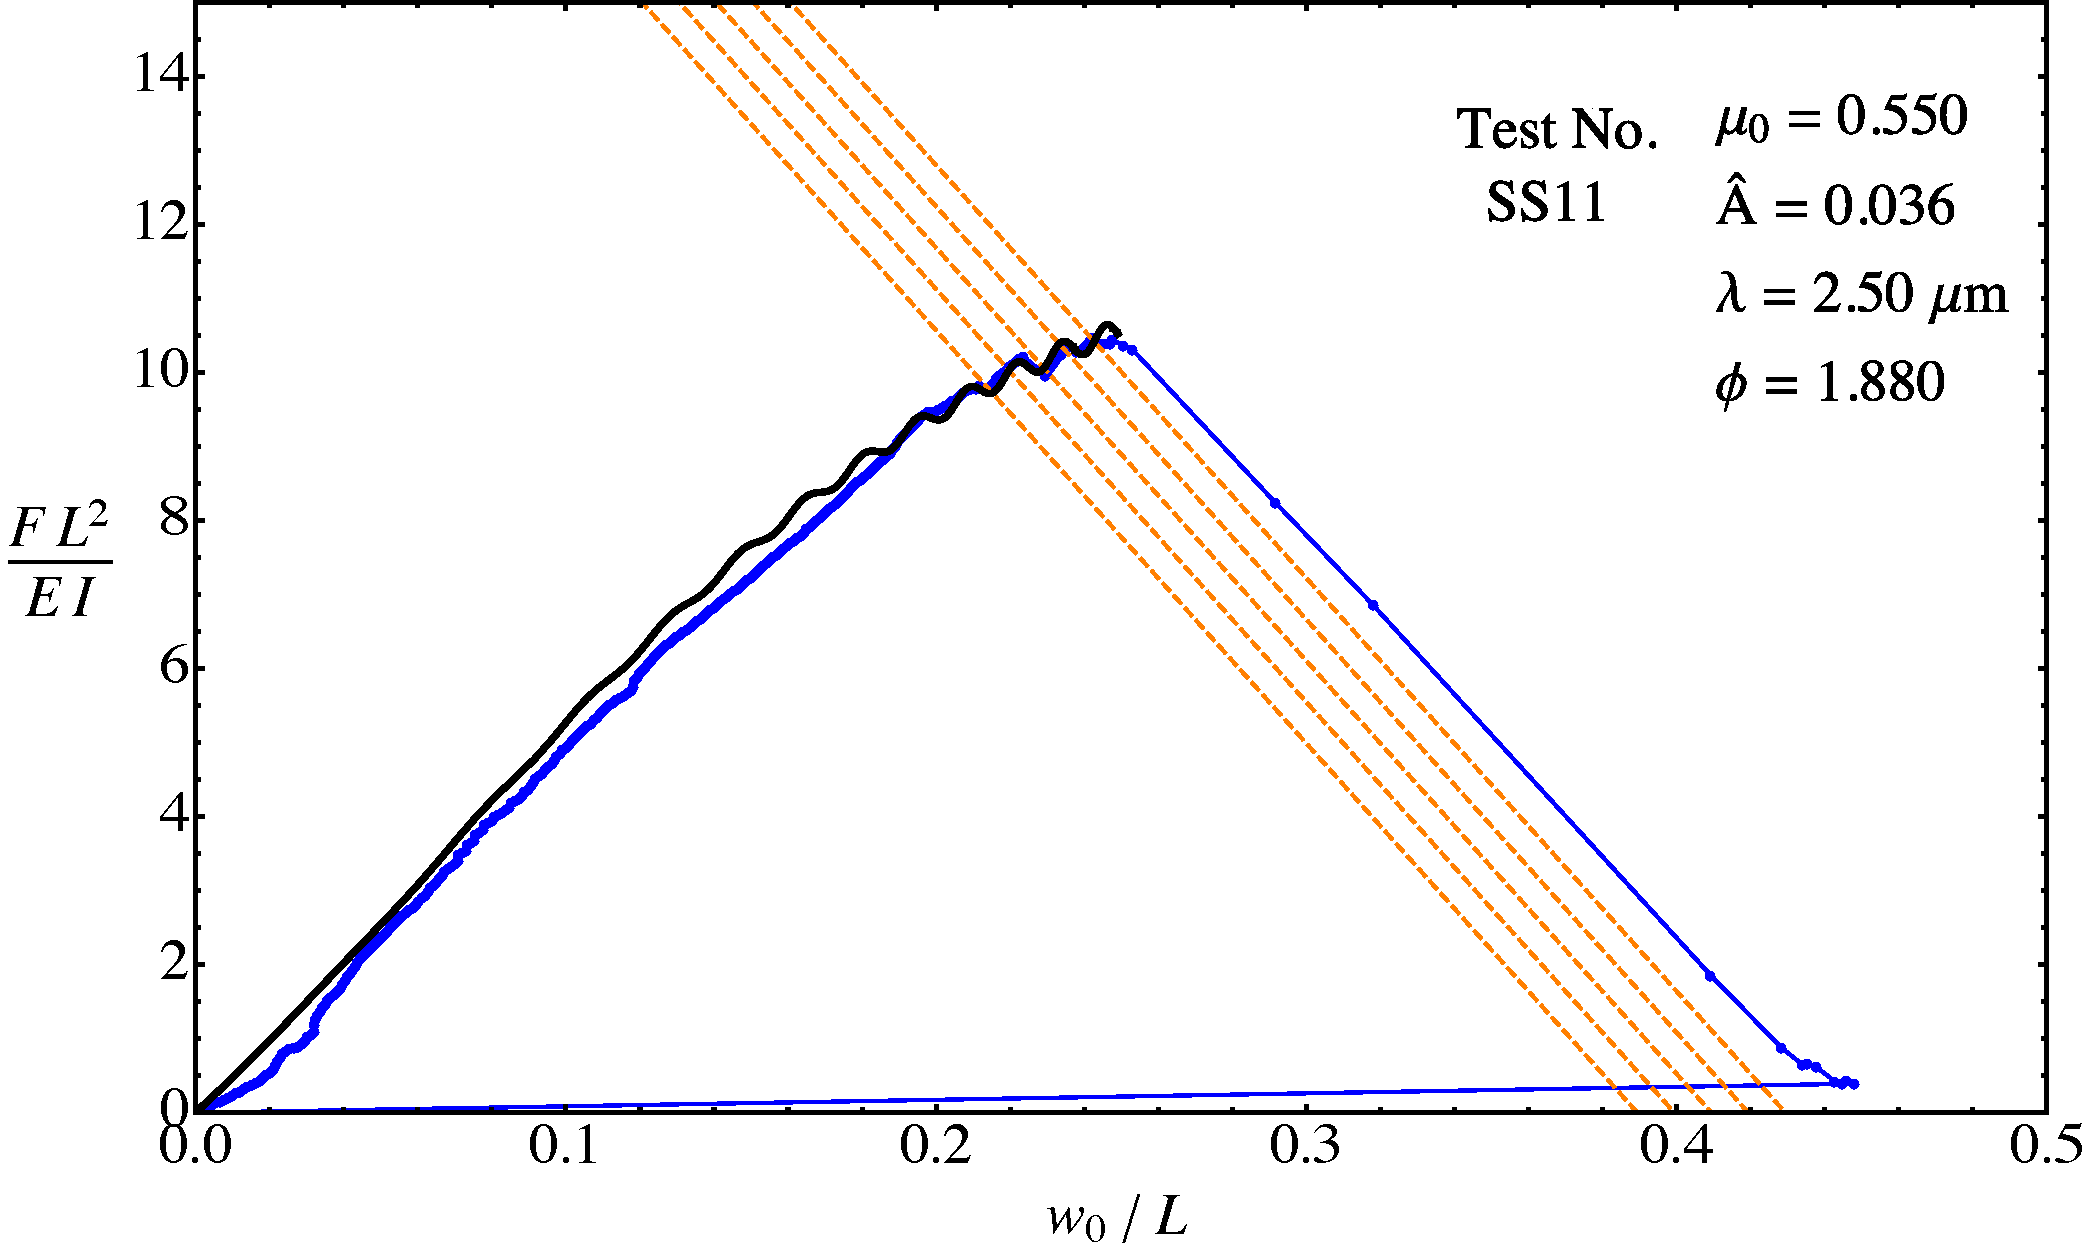
\includegraphics[width = .5\linewidth]{Figures/ComparisonThreeModels/Fitting05.pdf}}
\subfigure{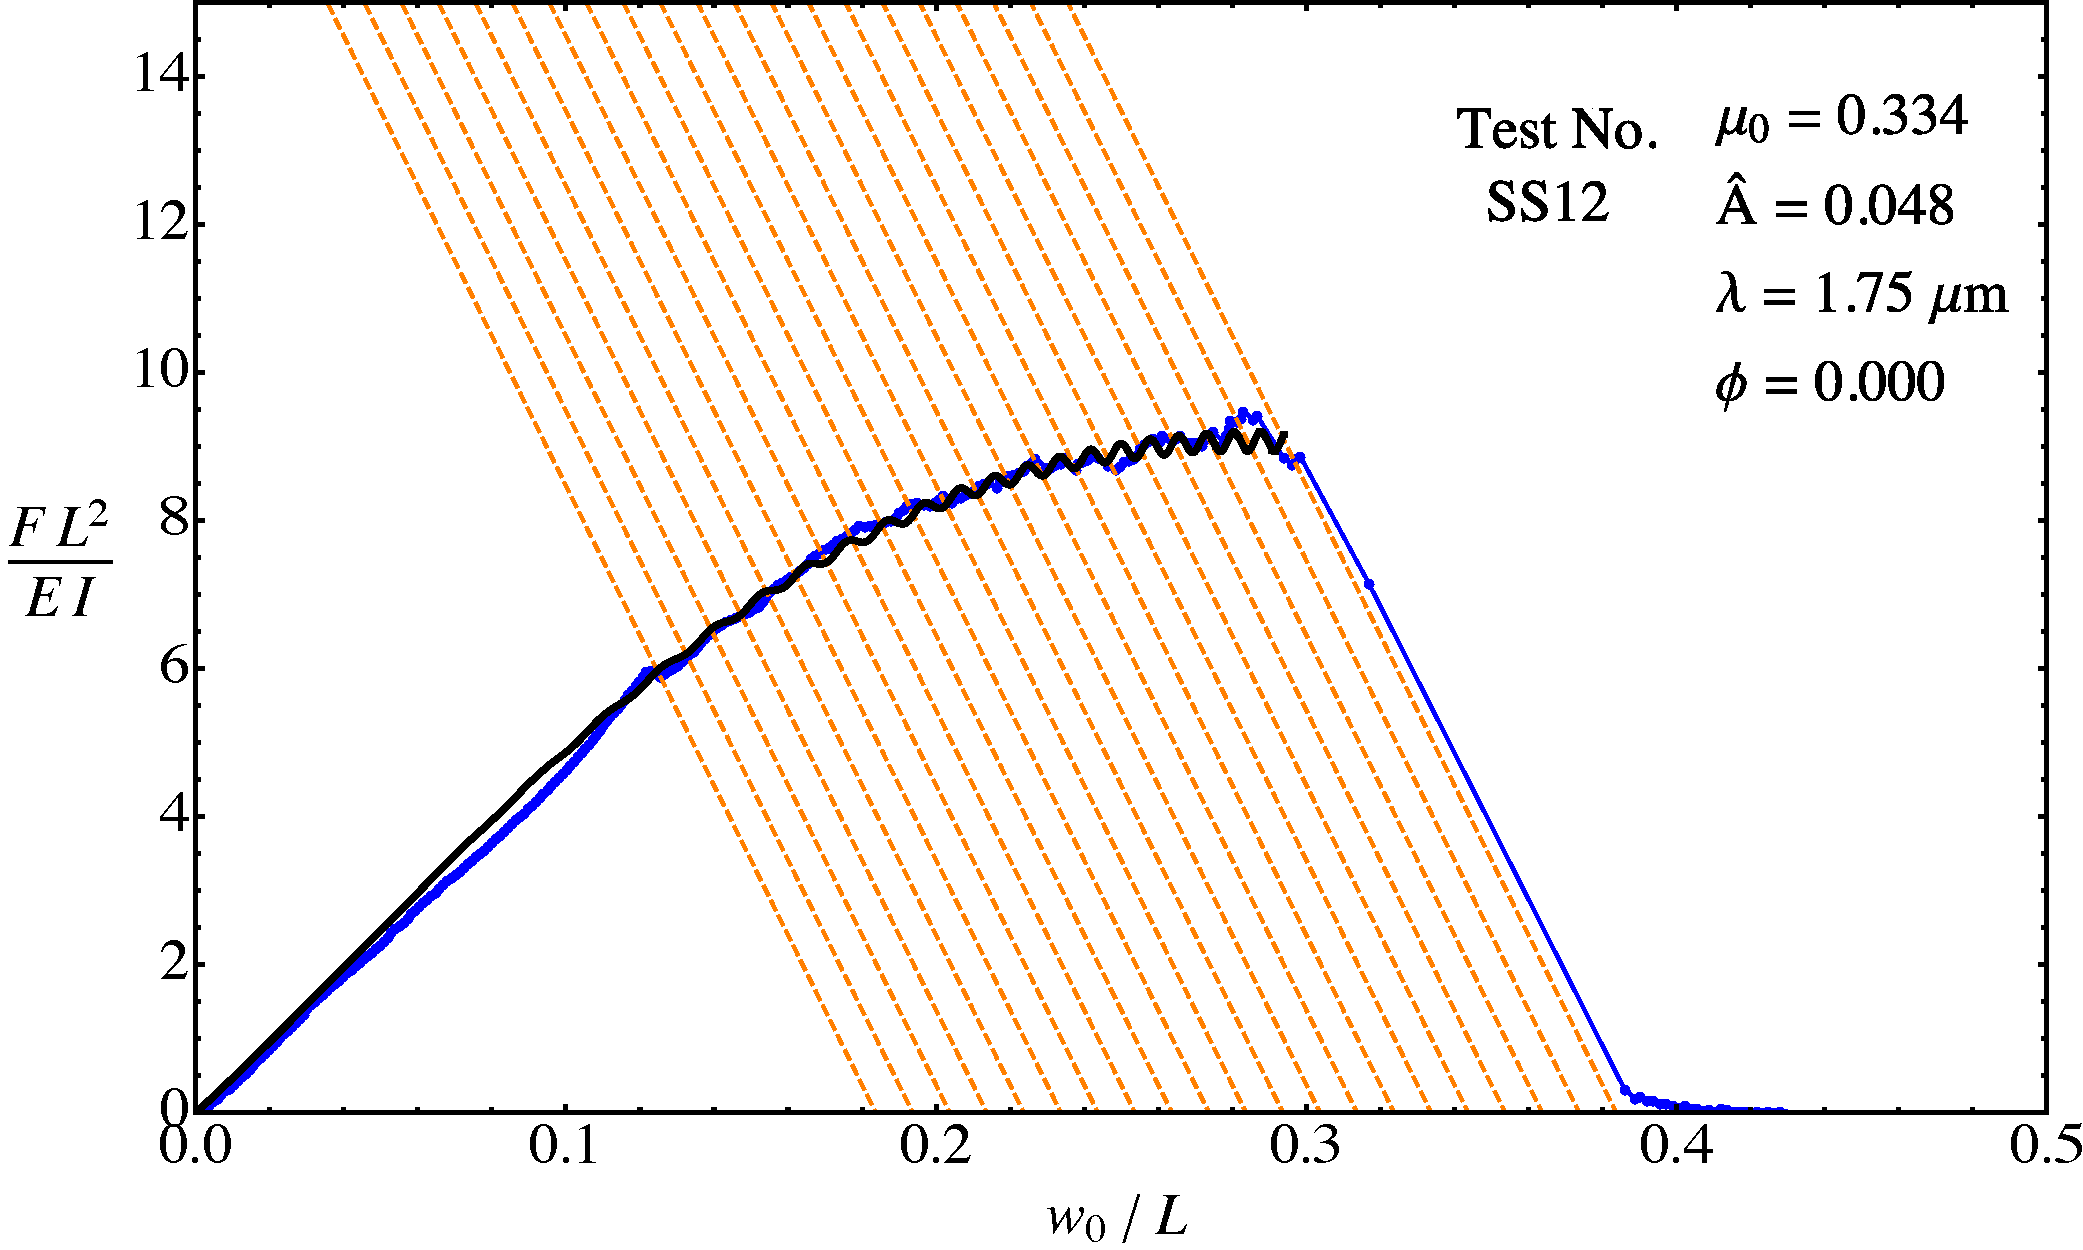
\includegraphics[width = .5\linewidth]{Figures/ComparisonThreeModels/Fitting06.pdf}}
\subfigure{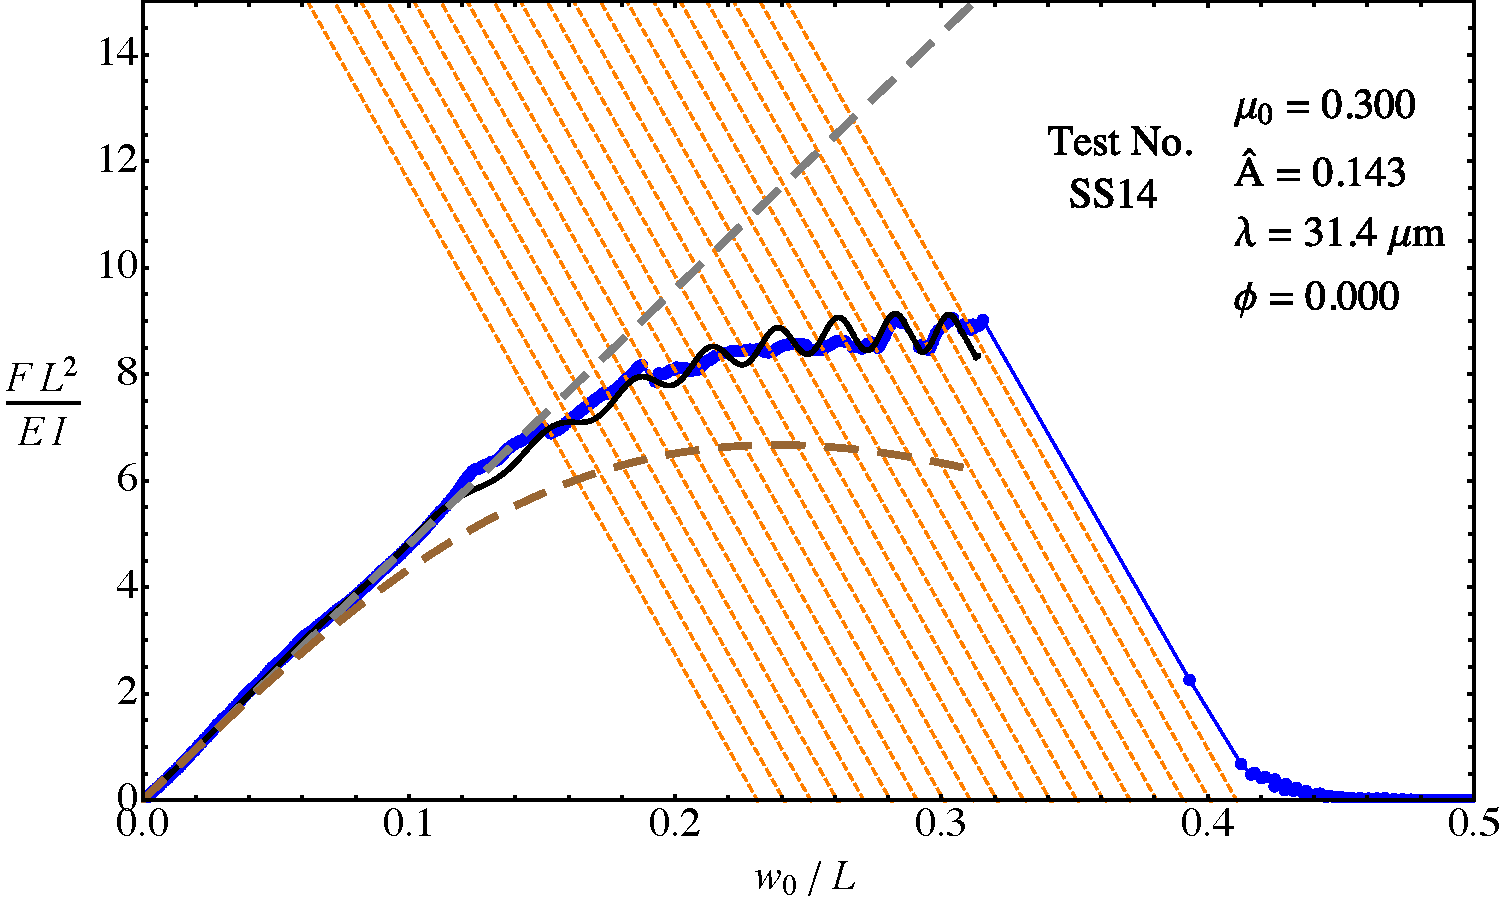
\includegraphics[width = .5\linewidth]{Figures/ComparisonThreeModels/Fitting07.pdf}}
\subfigure{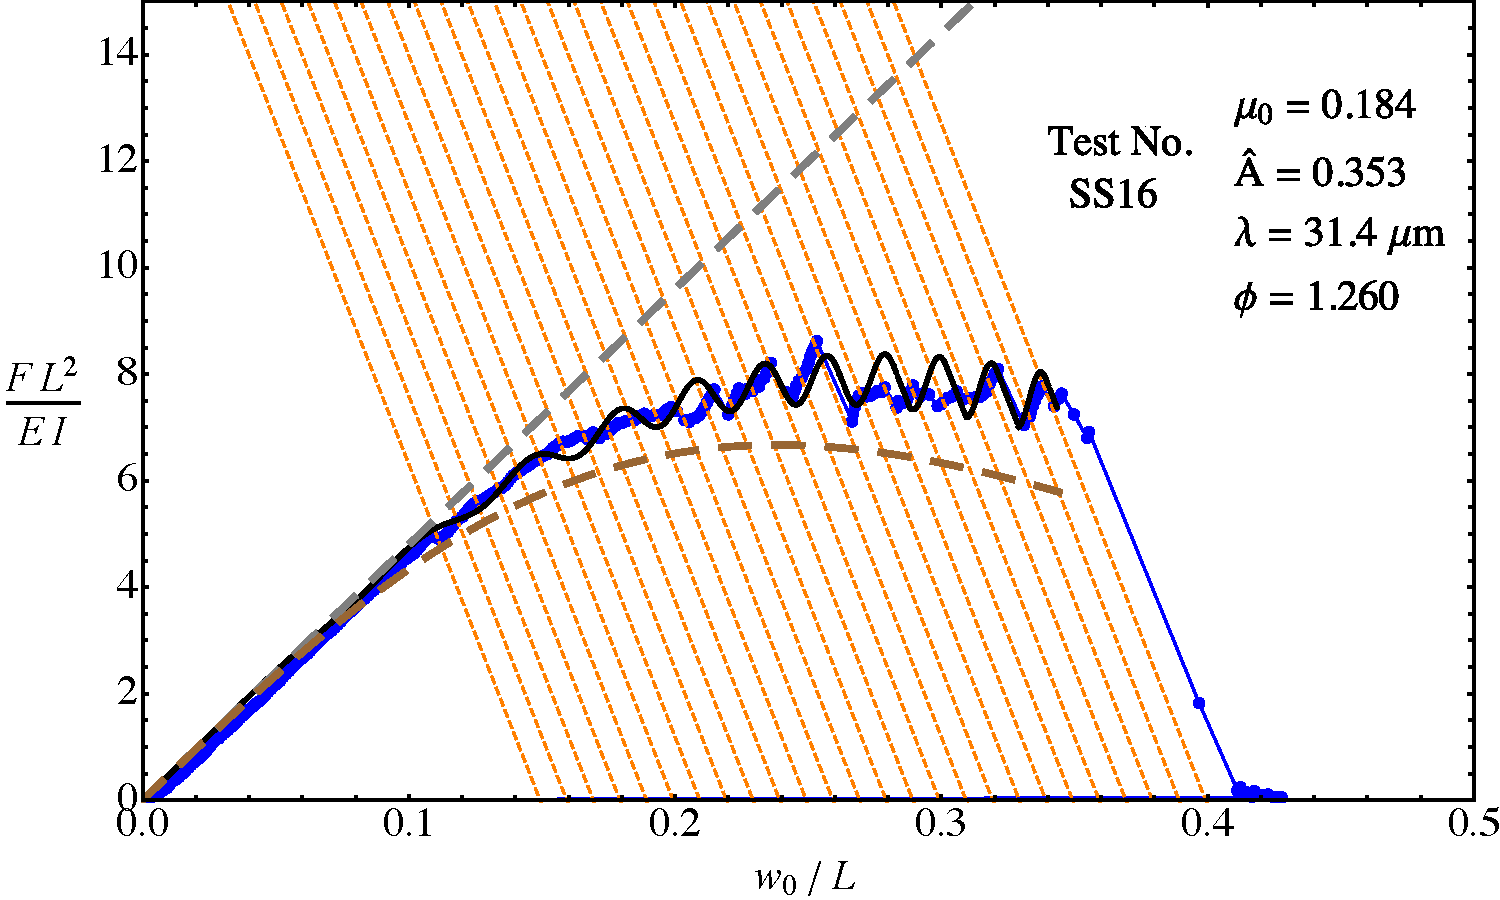
\includegraphics[width = .5\linewidth]{Figures/ComparisonThreeModels/Fitting08.pdf}}
\caption{Comparisons between the theoretical (black) and experimental (blue) $\hat{F}$-$\hat{w}_0$ response for simply-supported tests with sawtooth pattern. The orange oblique lines describe the $\hat{F}$-$\hat{w}_0$ relations of the cantilever, the loading device in the test, as stage displacement $w_s$ increases.}
\end{figure}

\begin{figure}[H]
\subfigure{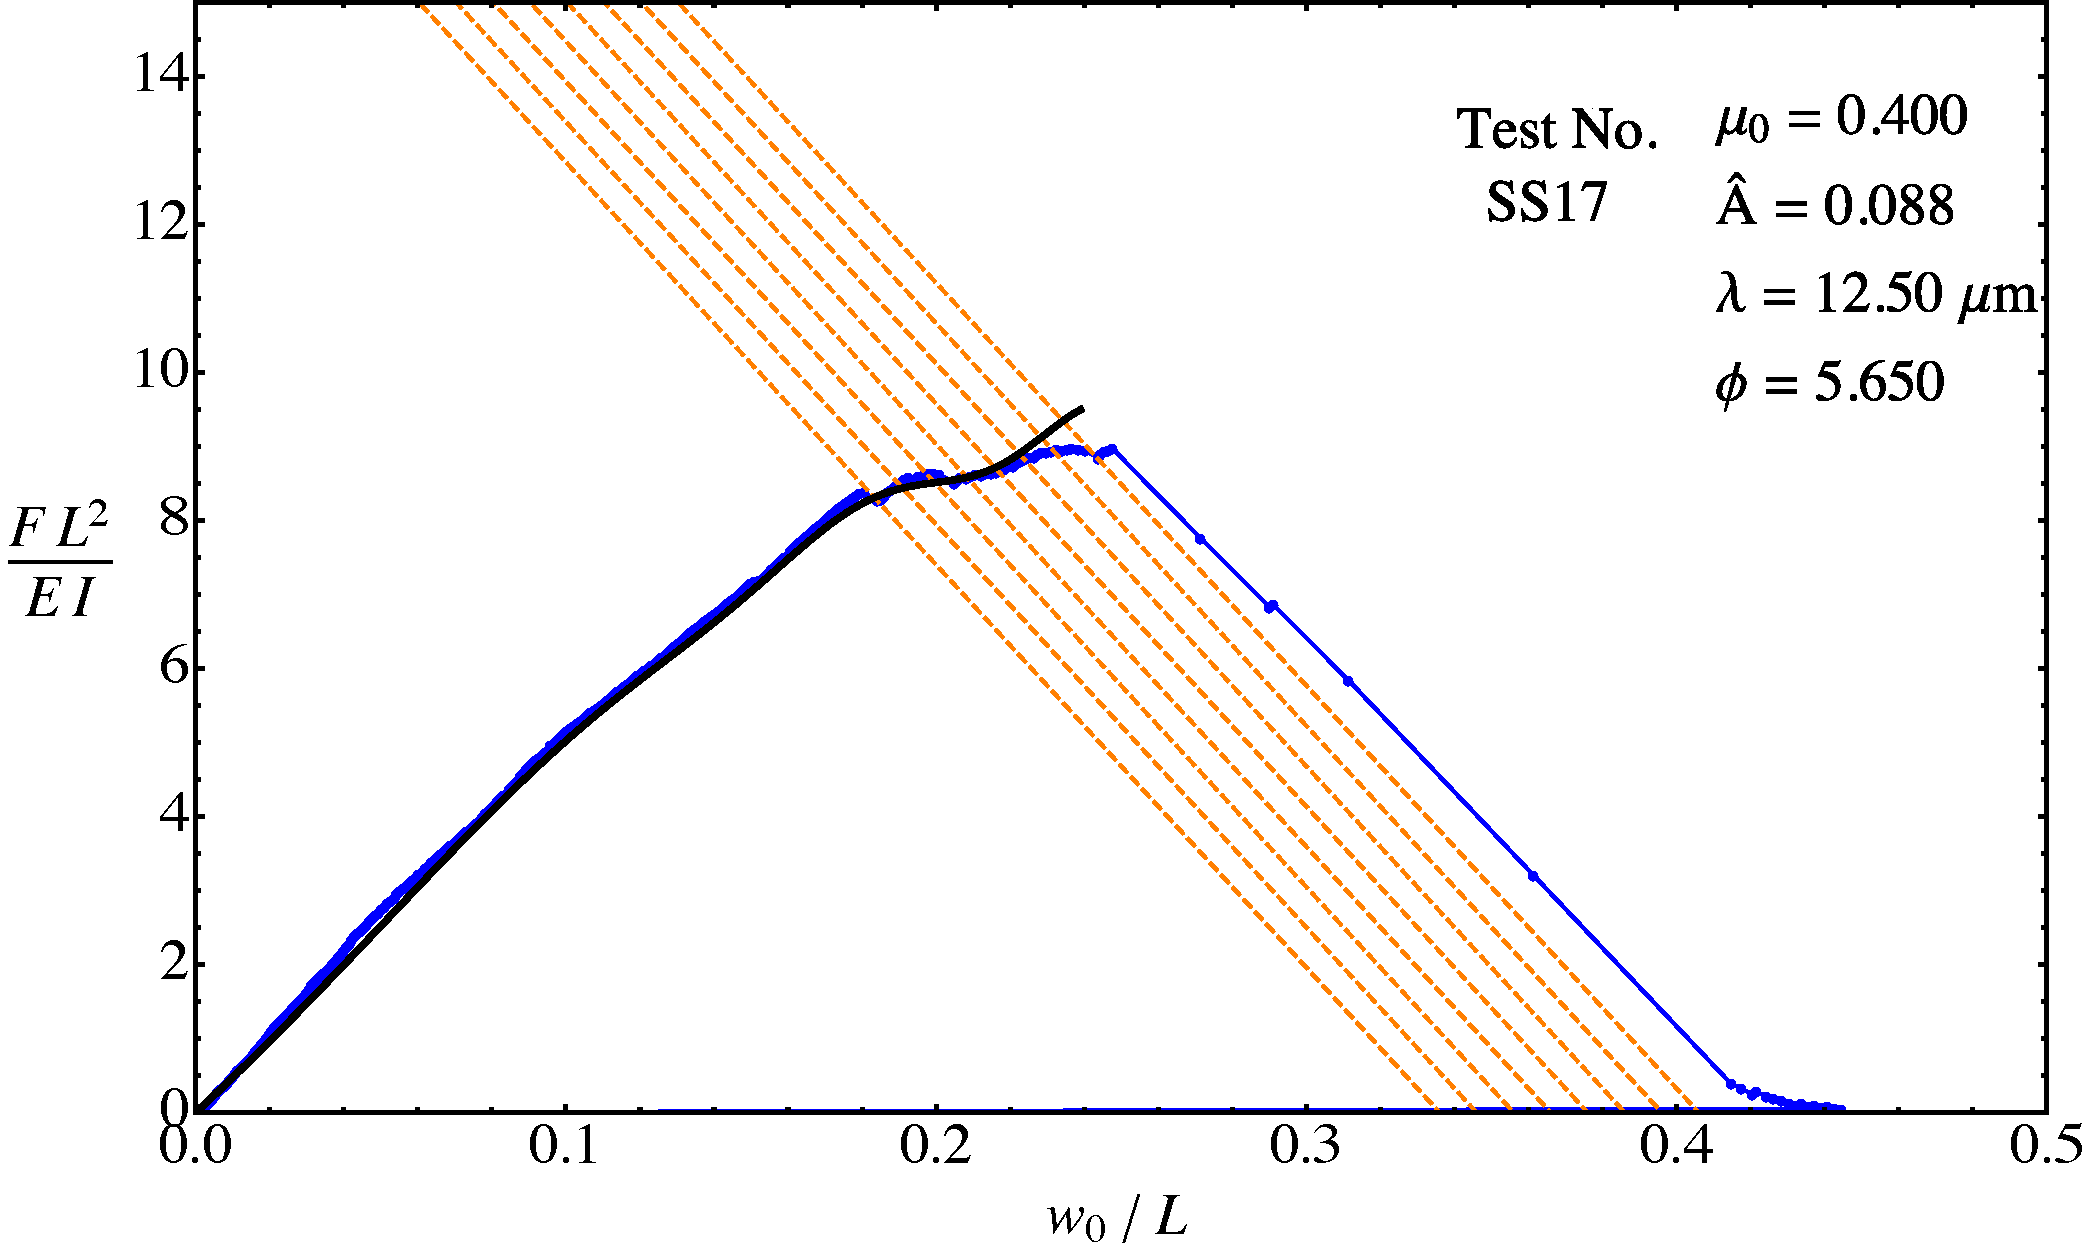
\includegraphics[width = .5\linewidth]{Figures/ComparisonThreeModels/Fitting09.pdf}}
\subfigure{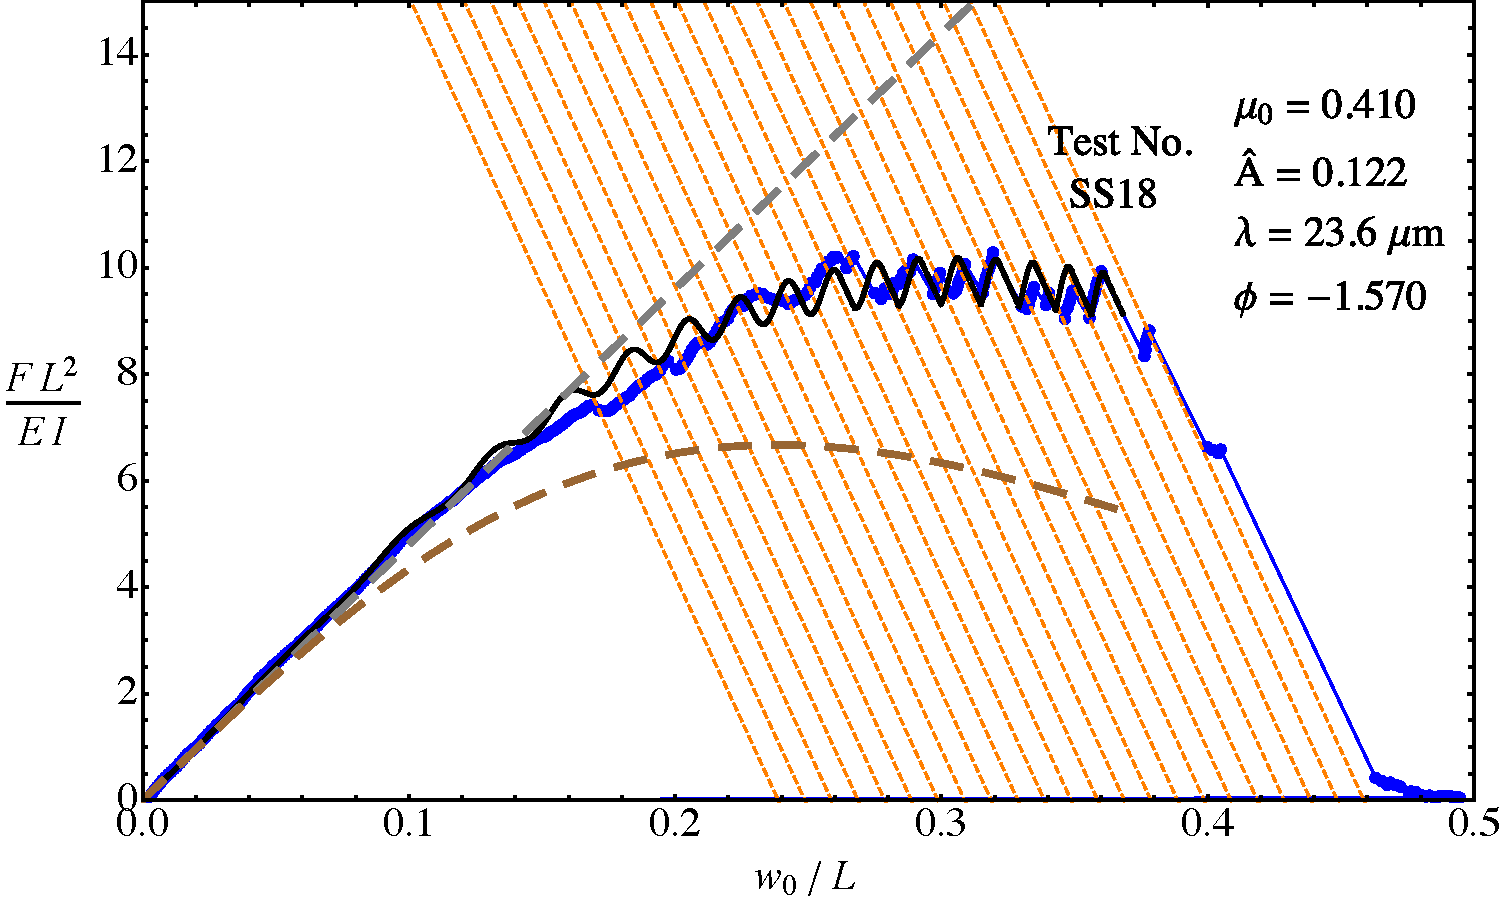
\includegraphics[width = .5\linewidth]{Figures/ComparisonThreeModels/Fitting10.pdf}}
\subfigure{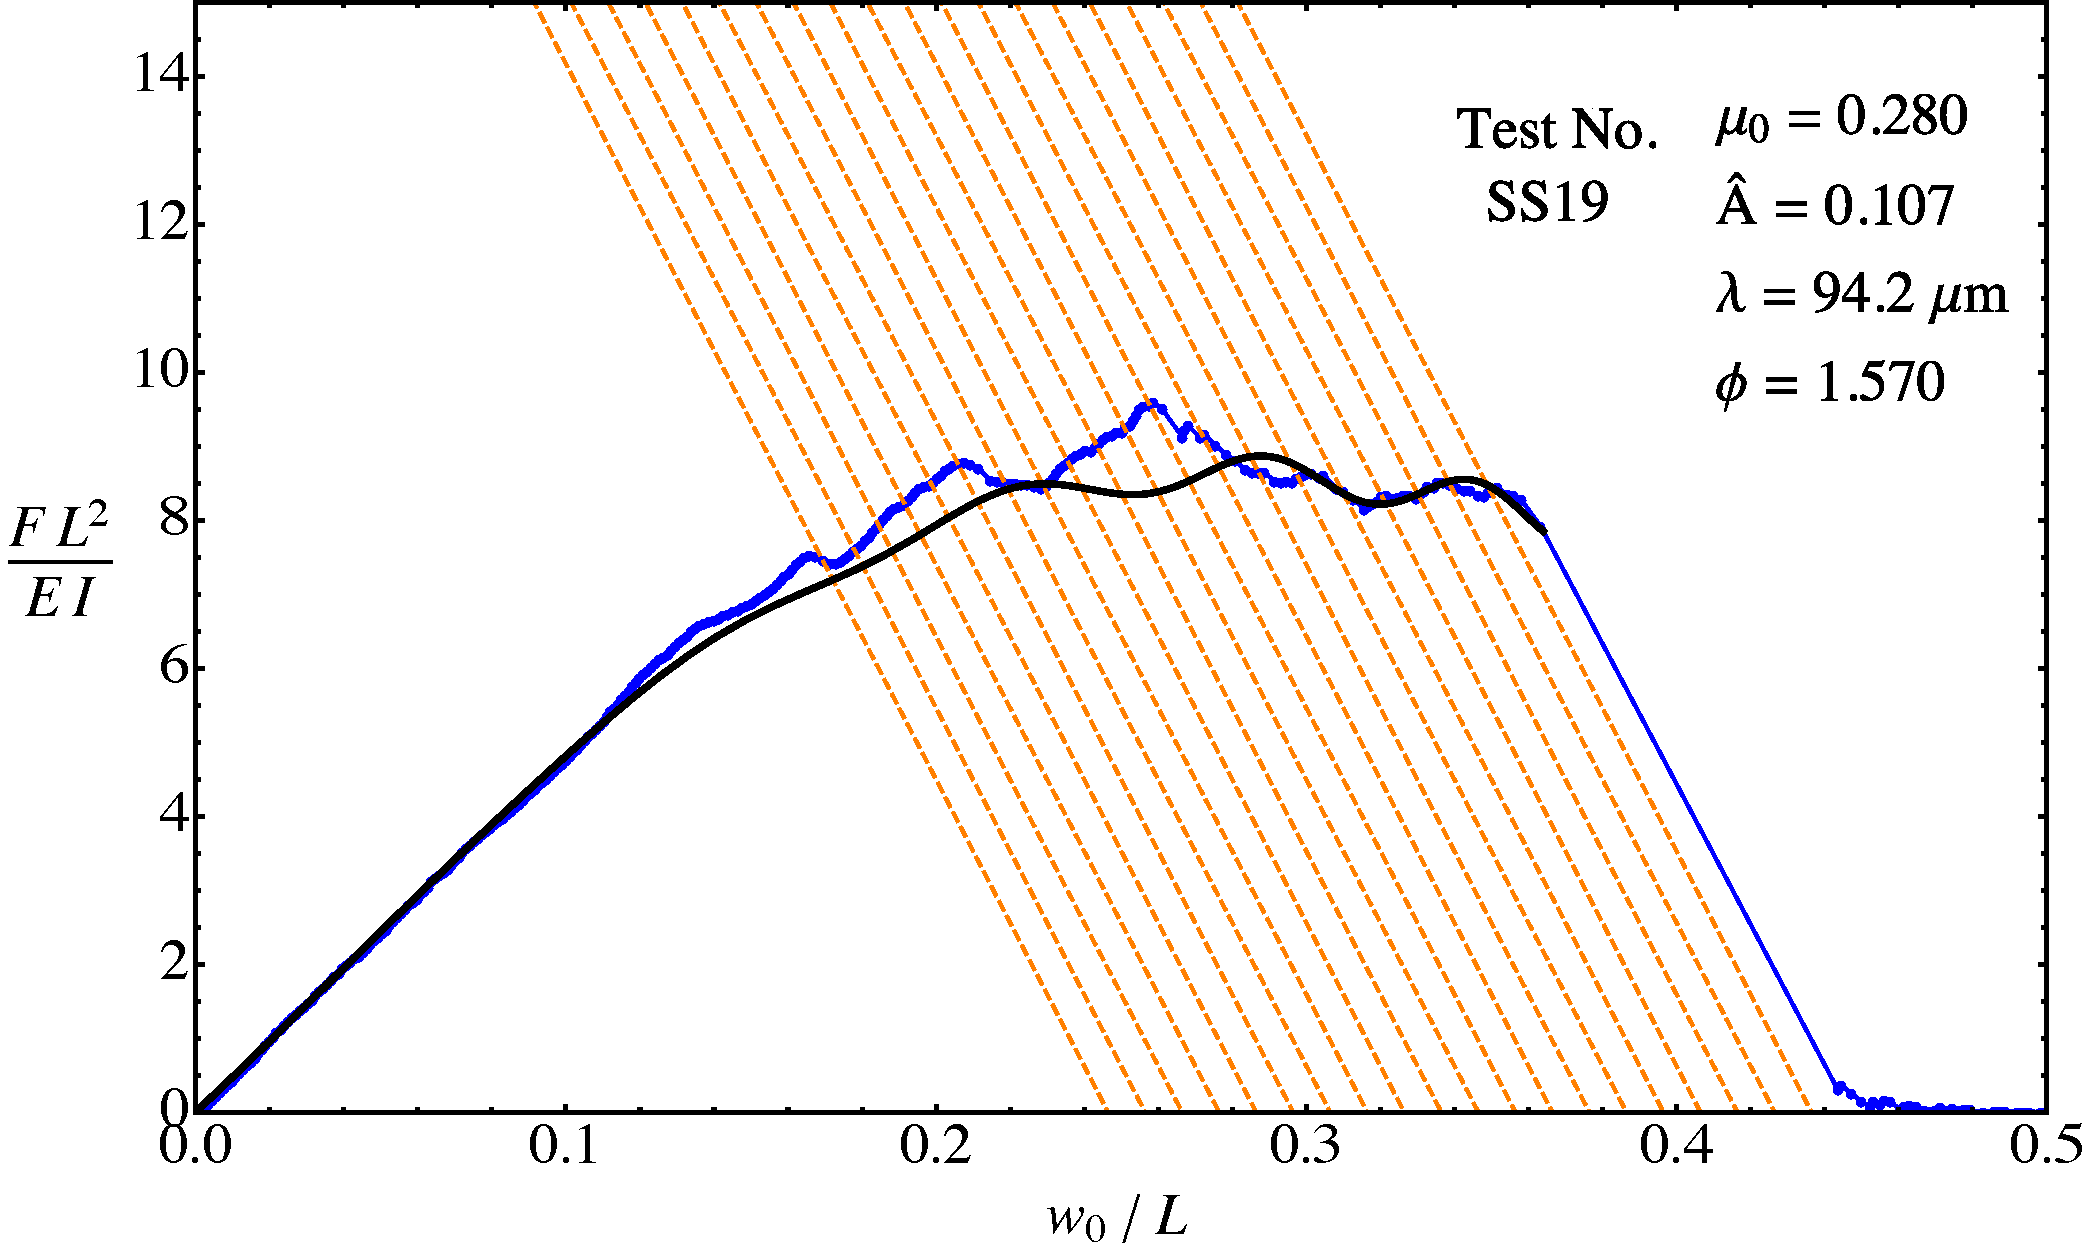
\includegraphics[width = .5\linewidth]{Figures/ComparisonThreeModels/Fitting11.pdf}}
\subfigure{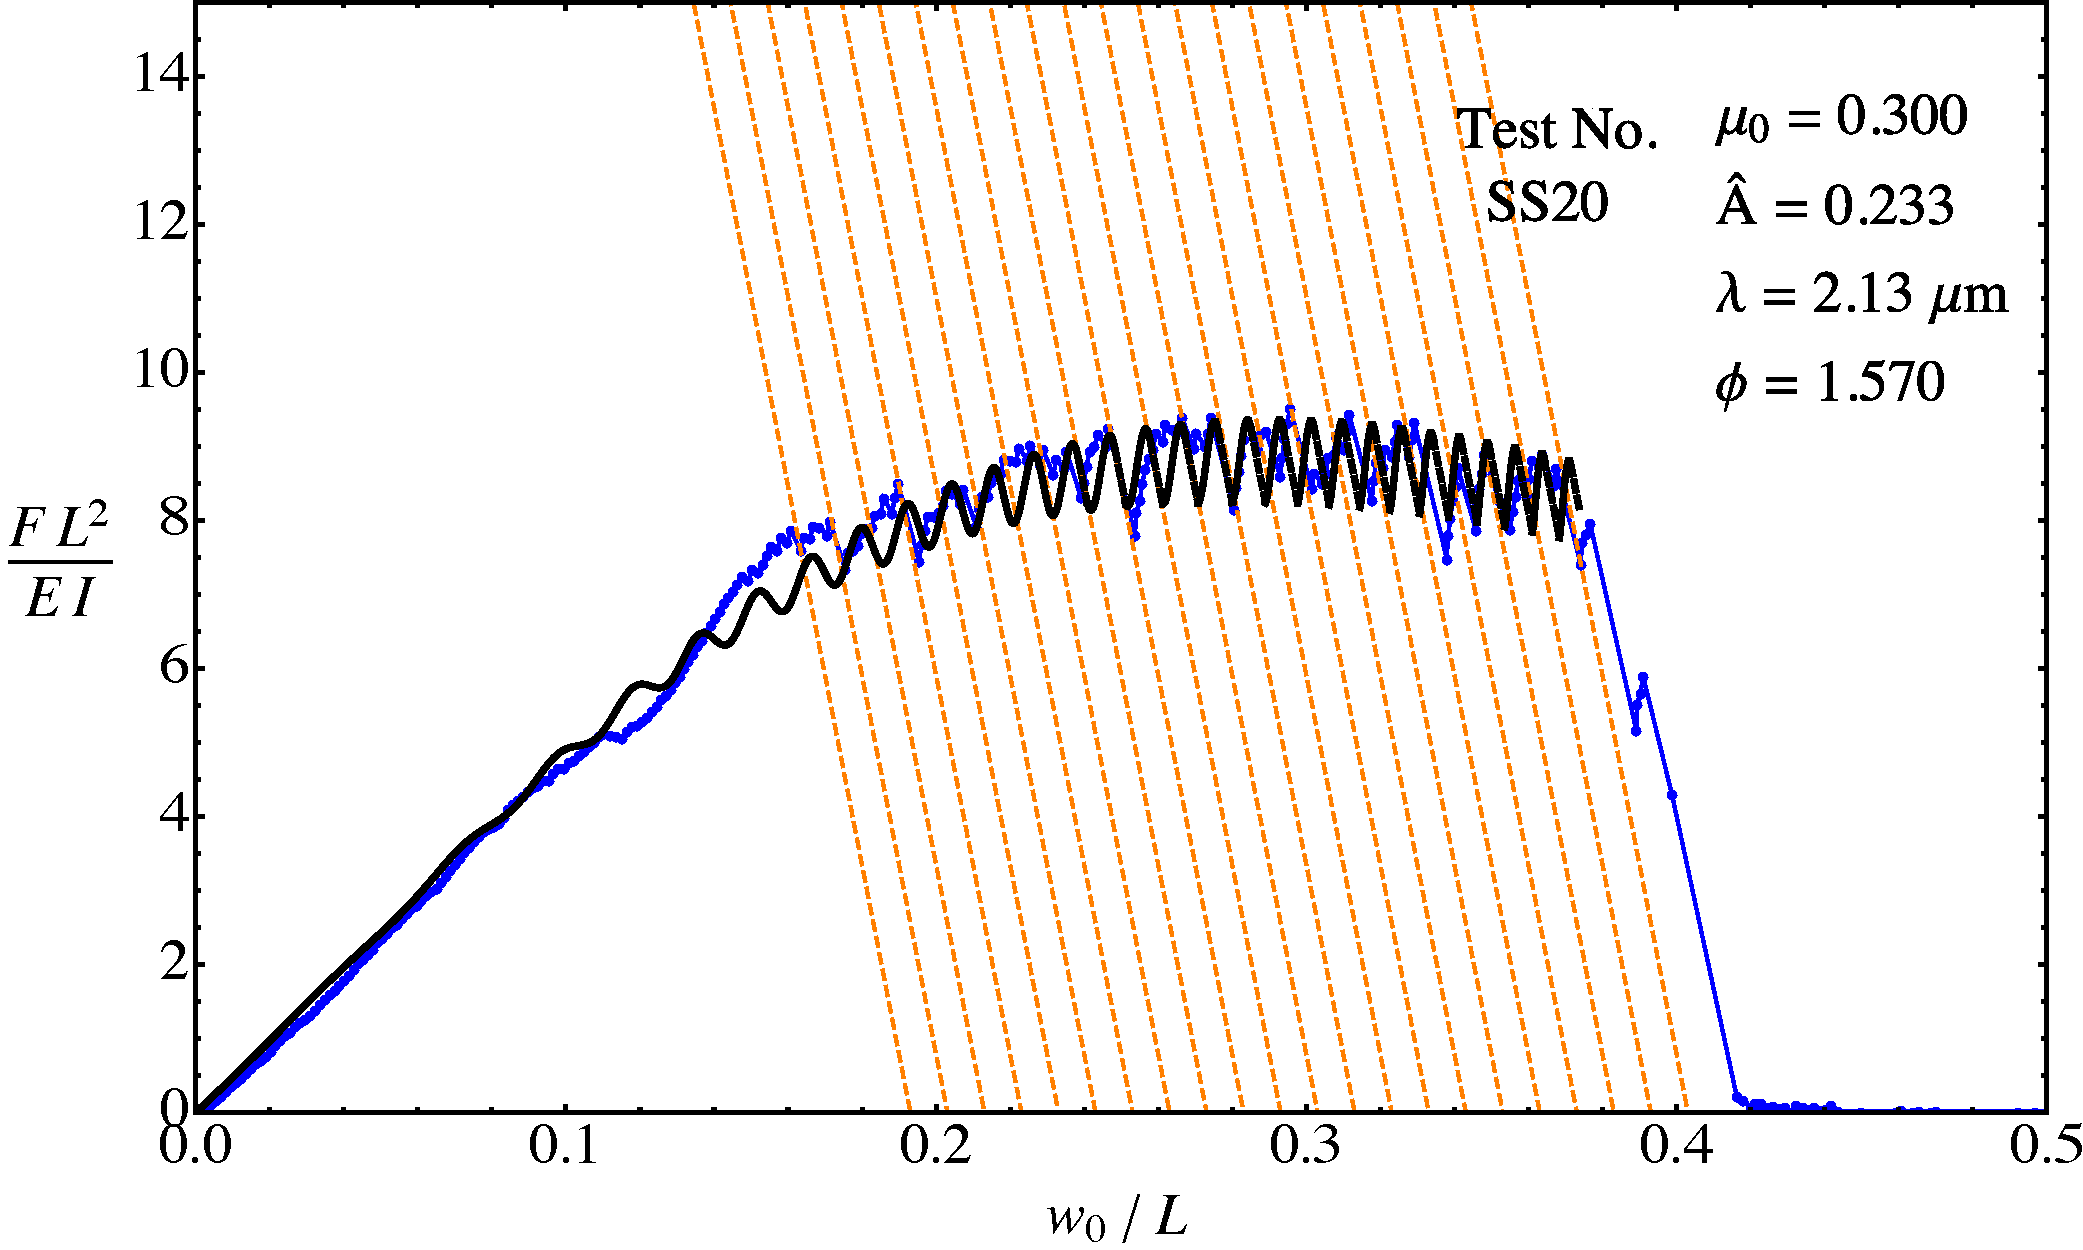
\includegraphics[width = .5\linewidth]{Figures/ComparisonThreeModels/Fitting12.pdf}}
\subfigure{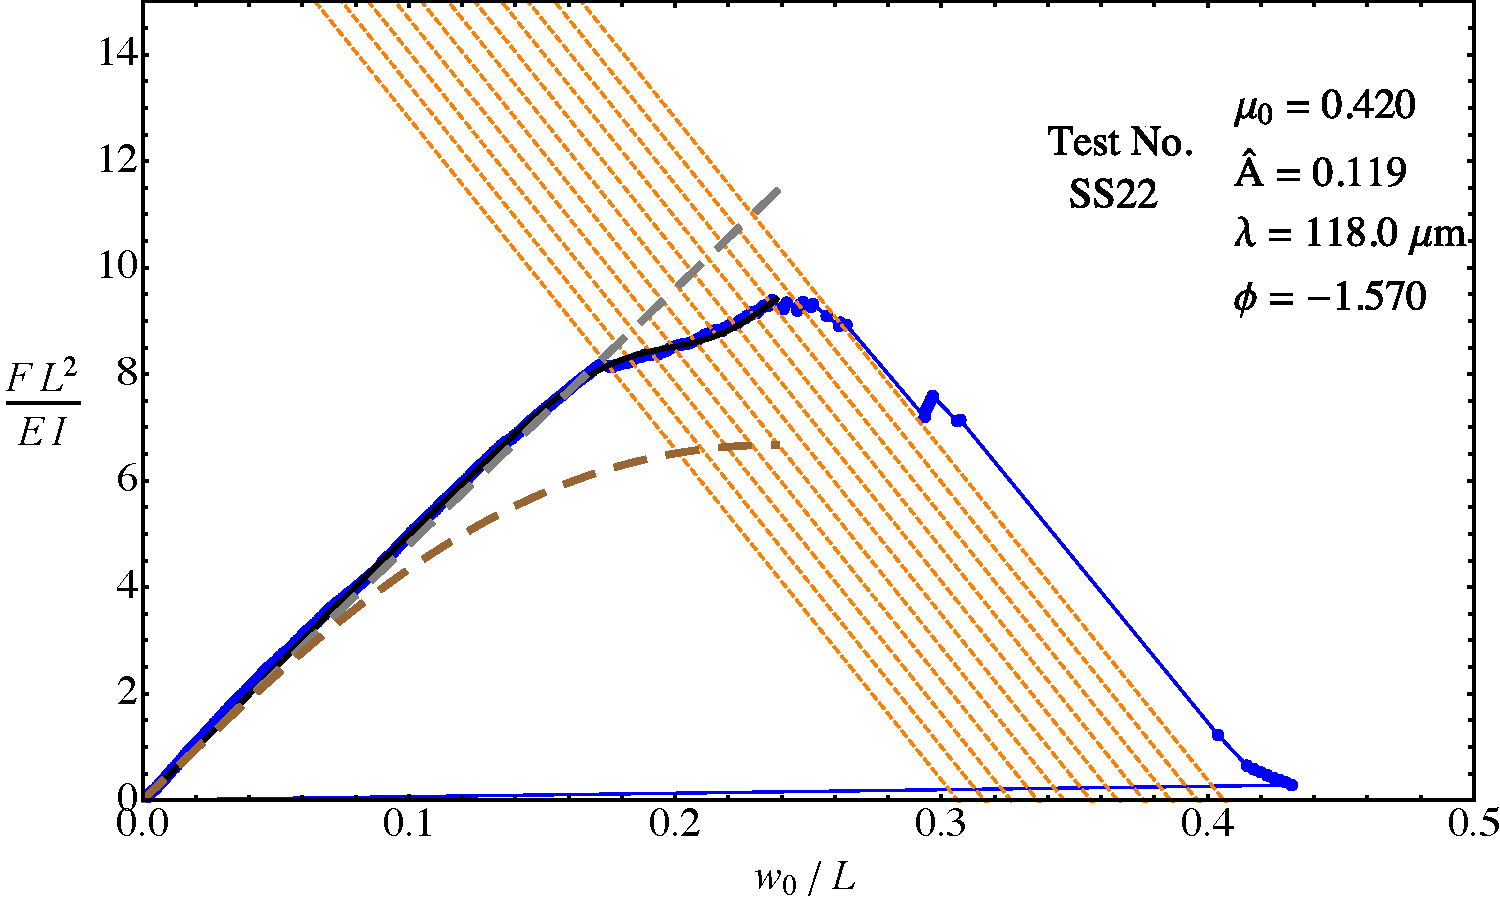
\includegraphics[width = .5\linewidth]{Figures/ComparisonThreeModels/Fitting13.pdf}}
\subfigure{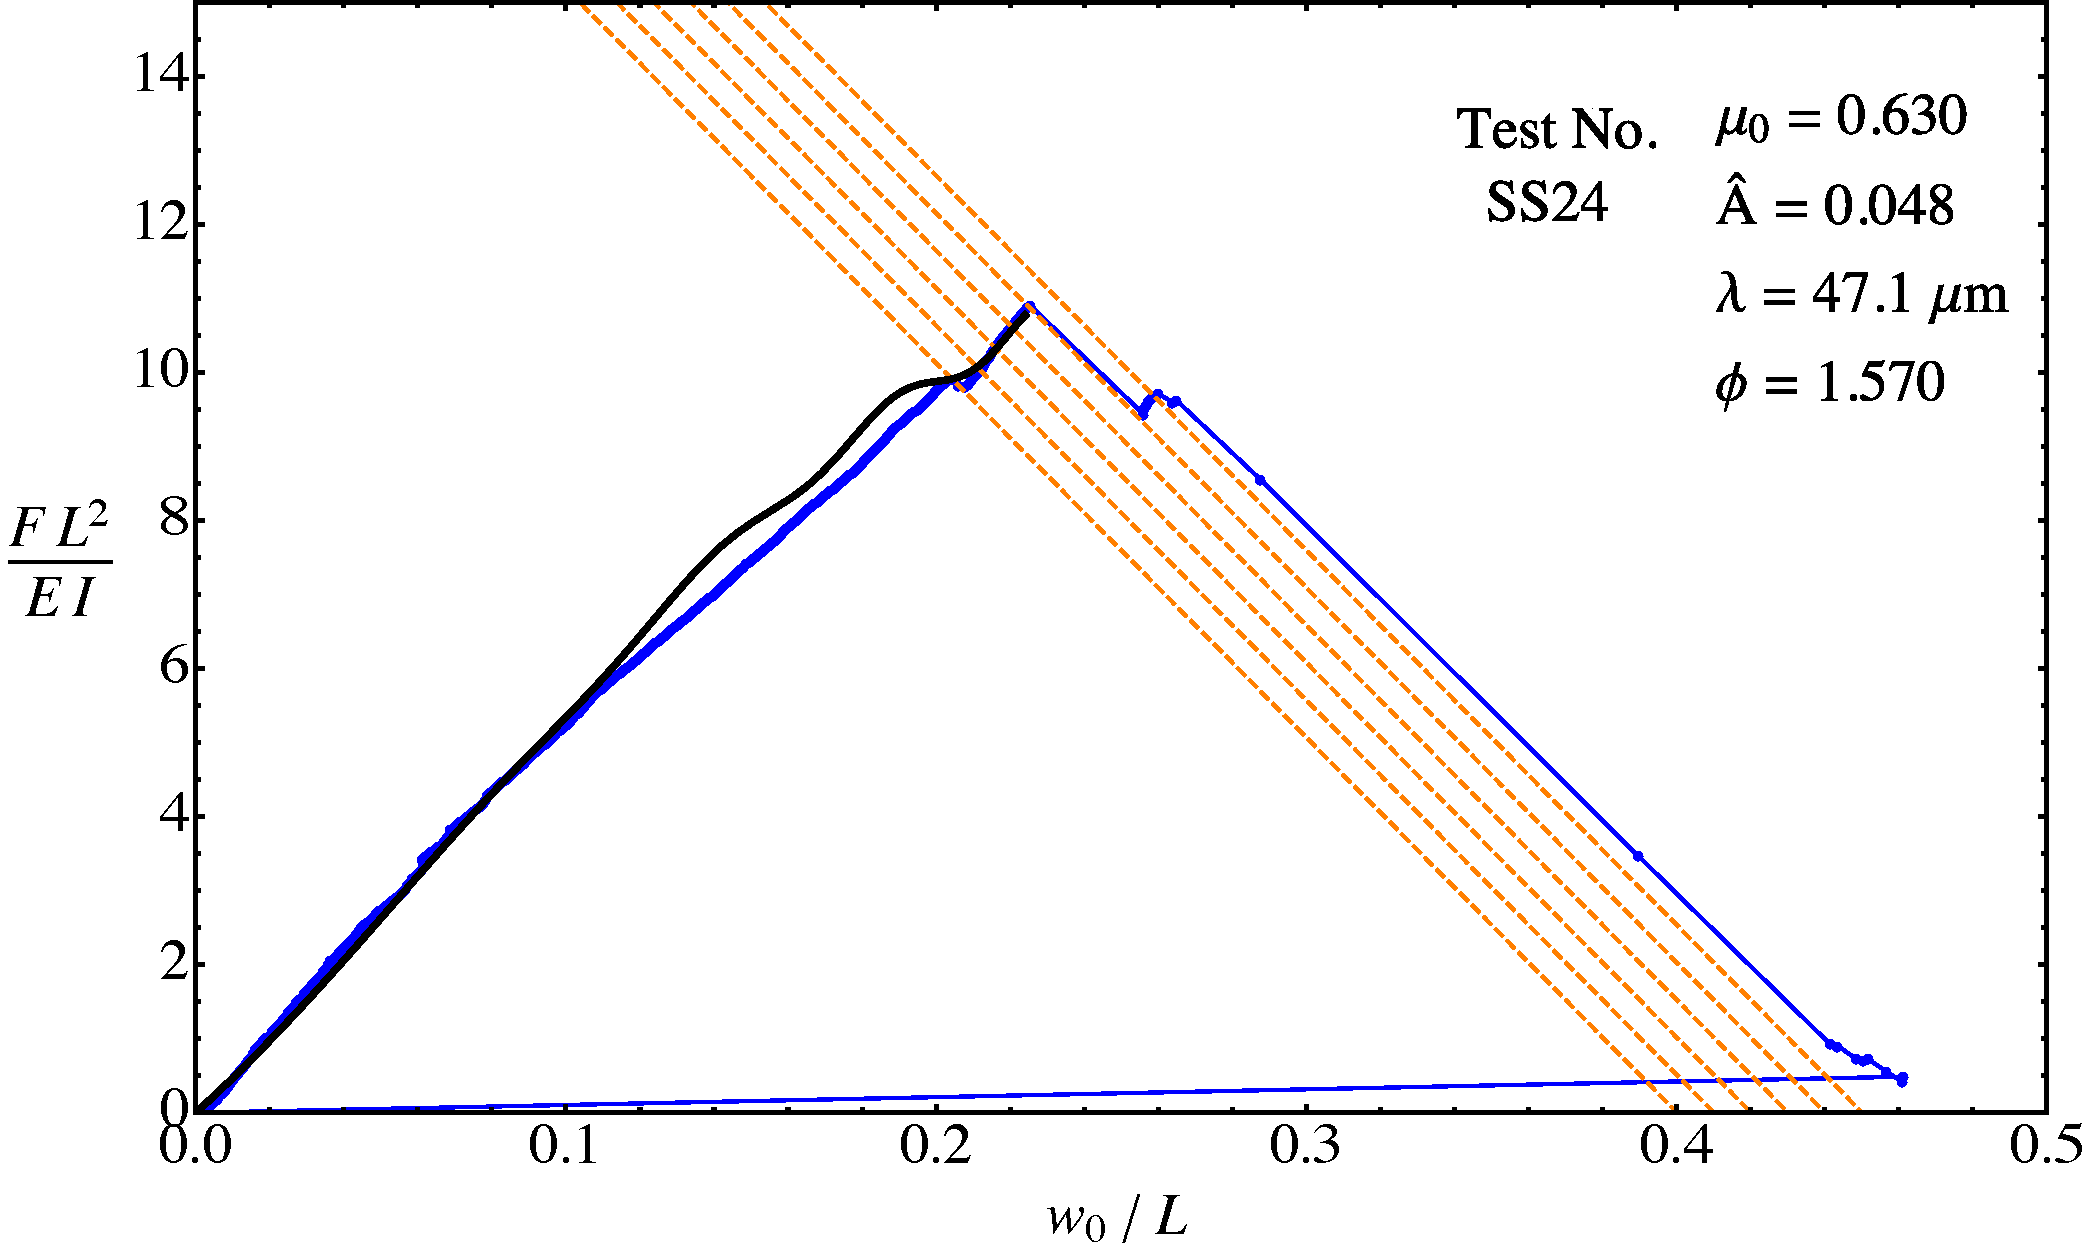
\includegraphics[width = .5\linewidth]{Figures/ComparisonThreeModels/Fitting14.pdf}}
\subfigure{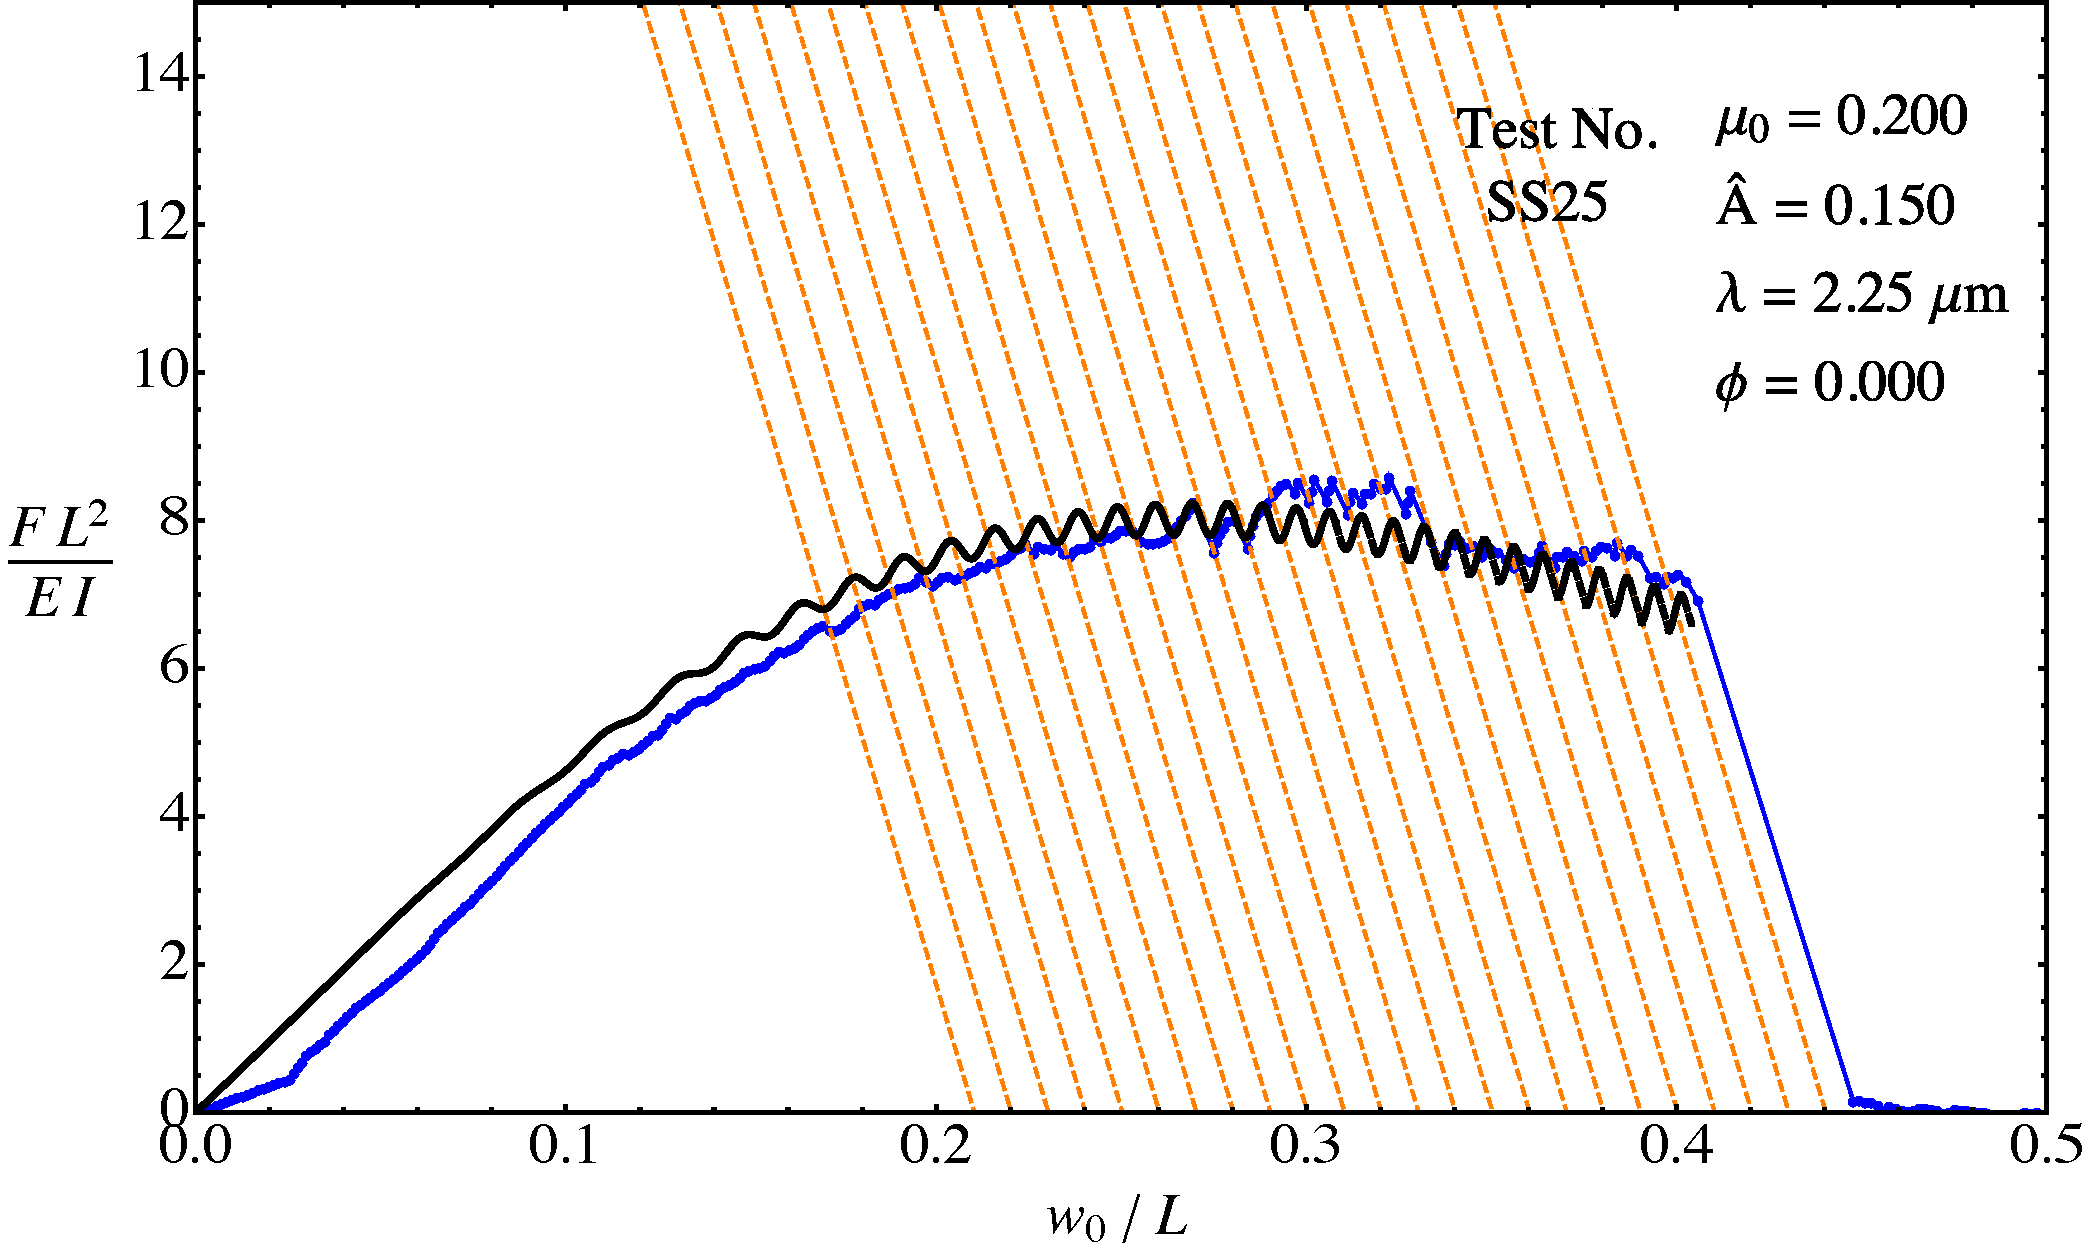
\includegraphics[width = .5\linewidth]{Figures/ComparisonThreeModels/Fitting15.pdf}}
\subfigure{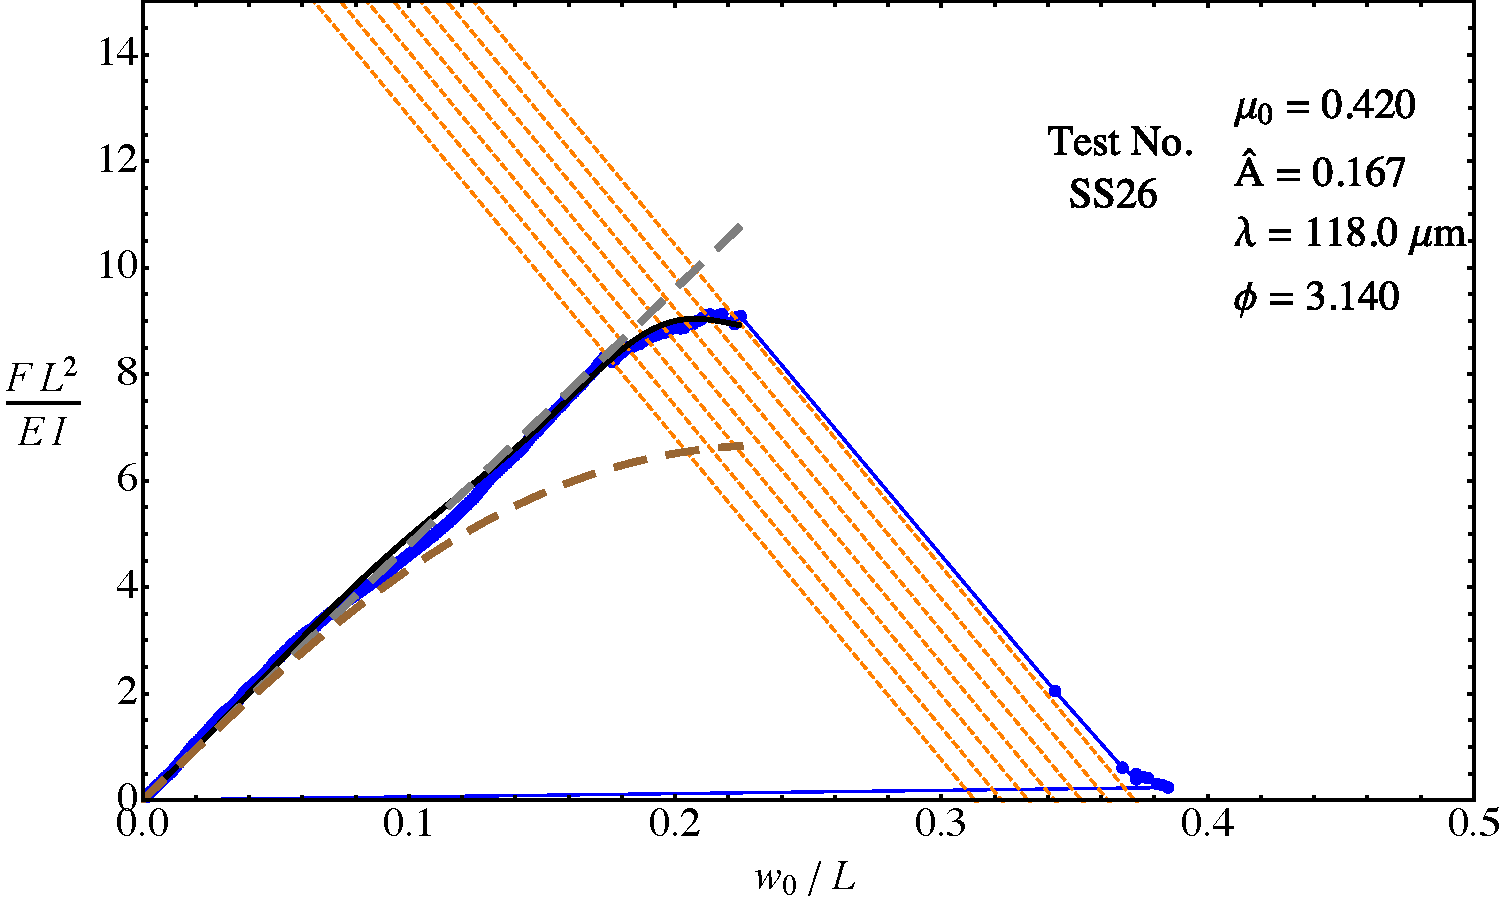
\includegraphics[width = .5\linewidth]{Figures/ComparisonThreeModels/Fitting16.pdf}}
\caption{Comparisons between the theoretical (black) and experimental (blue) $\hat{F}$-$\hat{w}_0$ response for simply-supported tests with sawtooth pattern (continued). The orange oblique lines describe the $\hat{F}$-$\hat{w}_0$ relations of the cantilever, the loading device in the test, as stage displacement $w_s$ increases.}
\end{figure}

\begin{figure}[H]
\subfigure{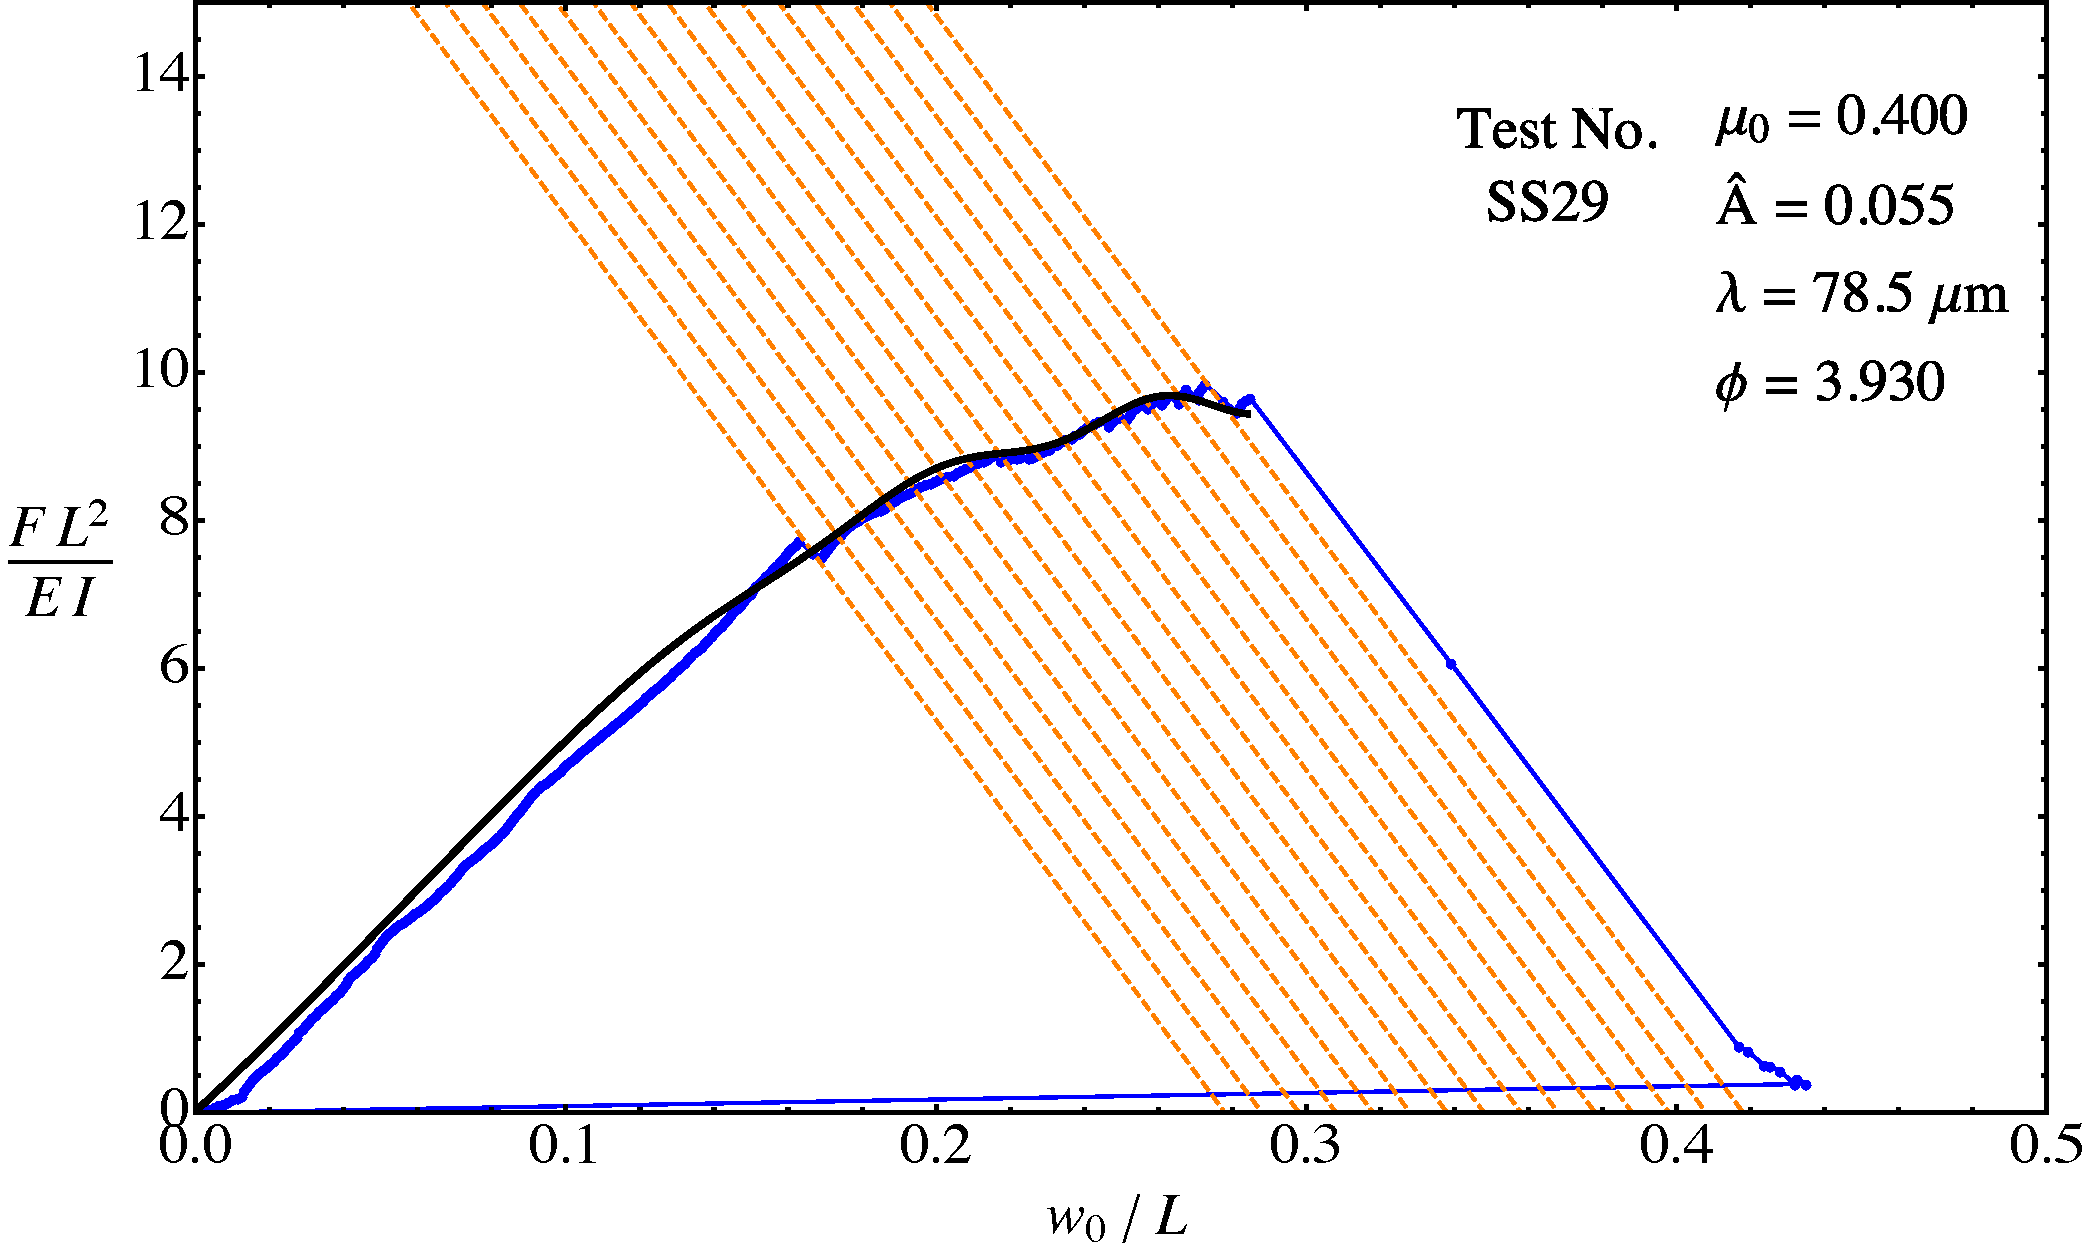
\includegraphics[width = .5\linewidth]{Figures/ComparisonThreeModels/Fitting17.pdf}}
\subfigure{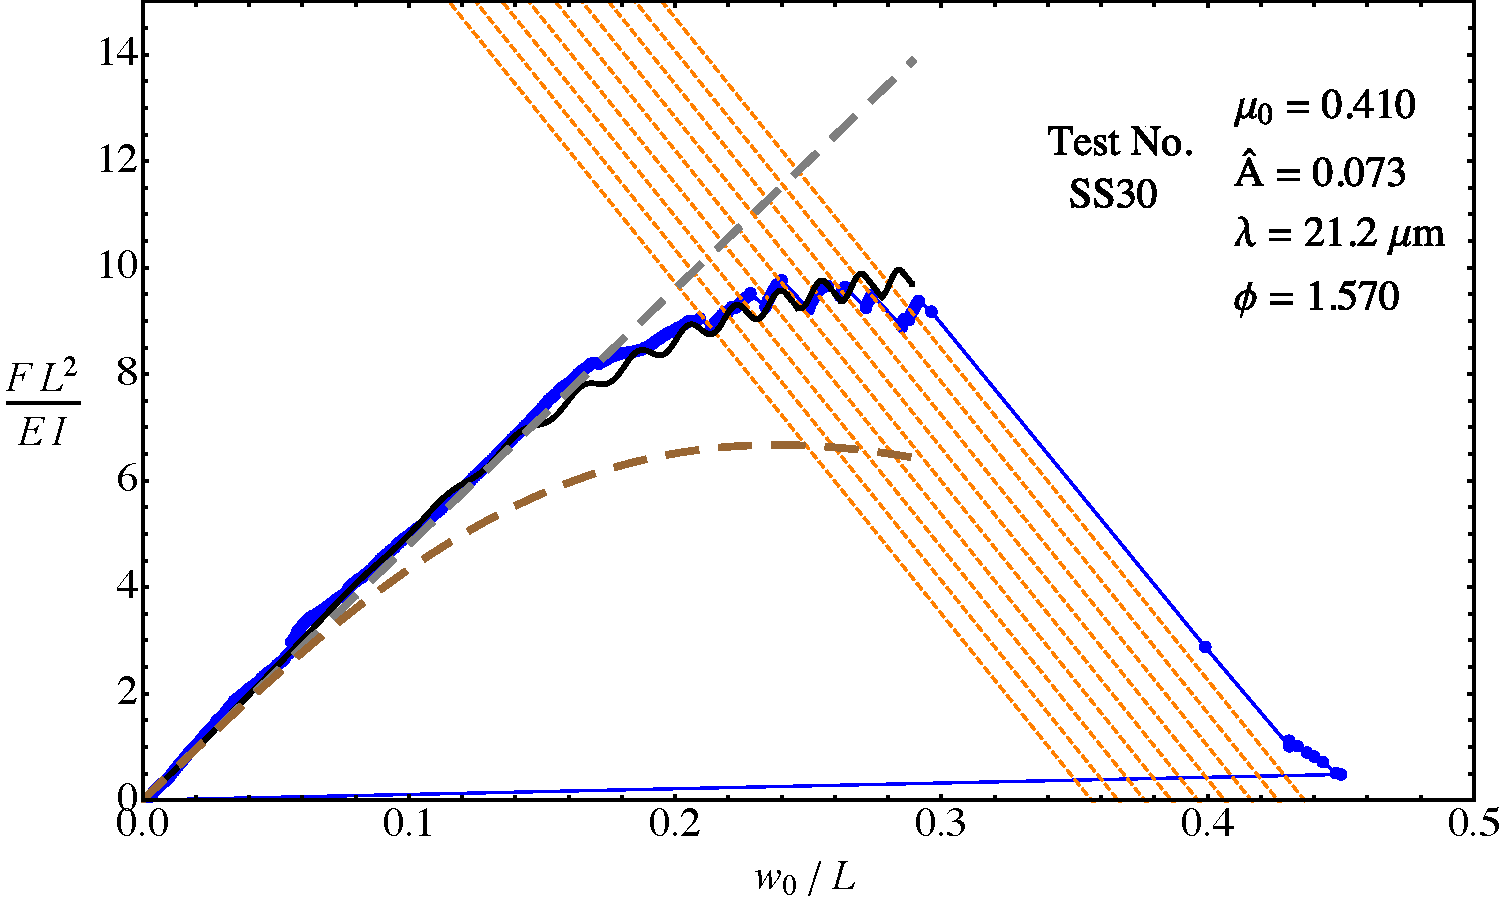
\includegraphics[width = .5\linewidth]{Figures/ComparisonThreeModels/Fitting18.pdf}}
\subfigure{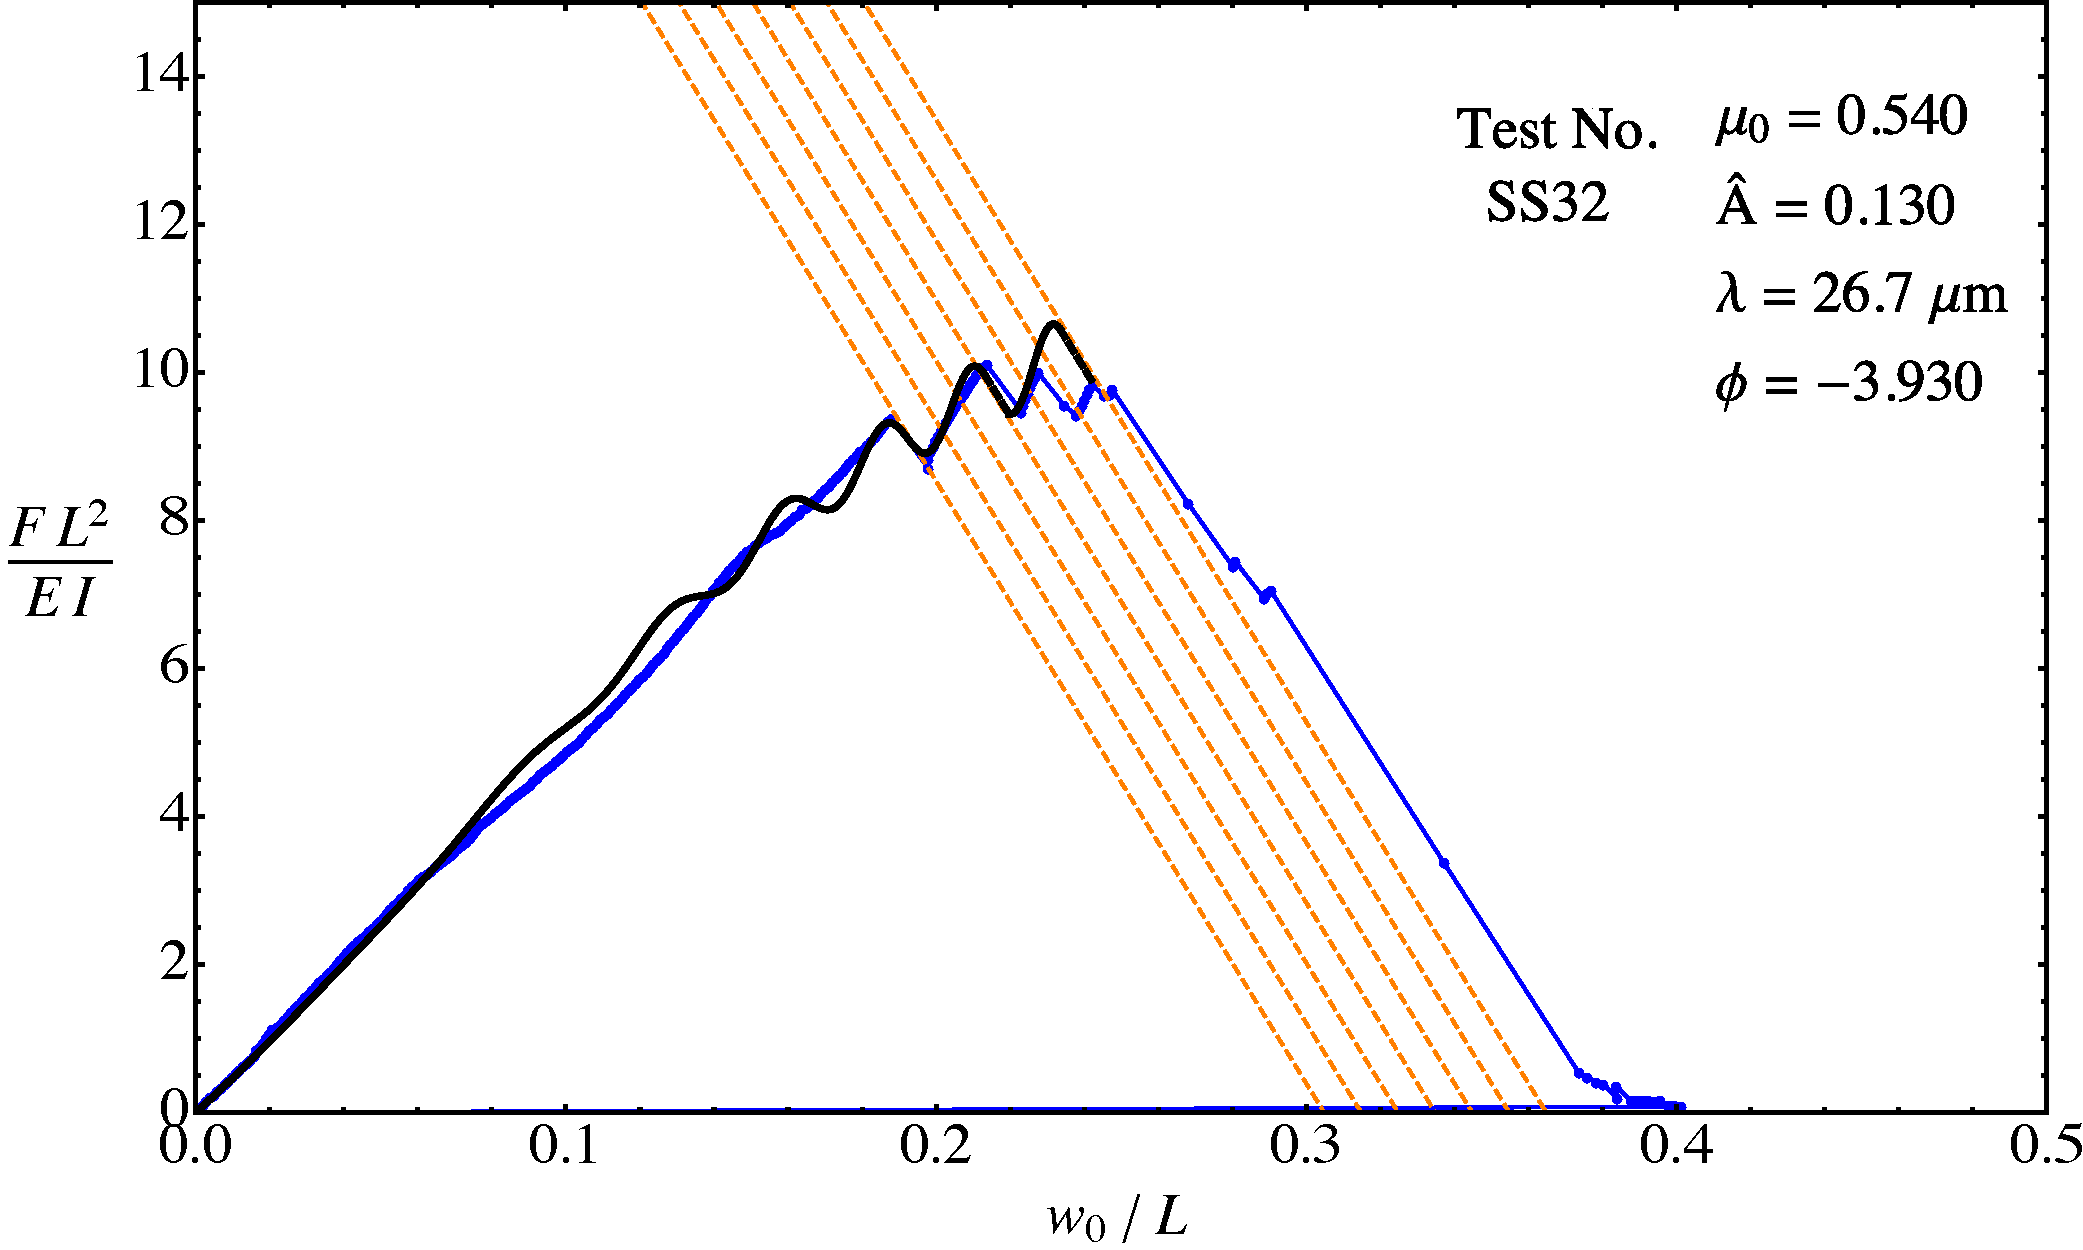
\includegraphics[width = .5\linewidth]{Figures/ComparisonThreeModels/Fitting19.pdf}}
\subfigure{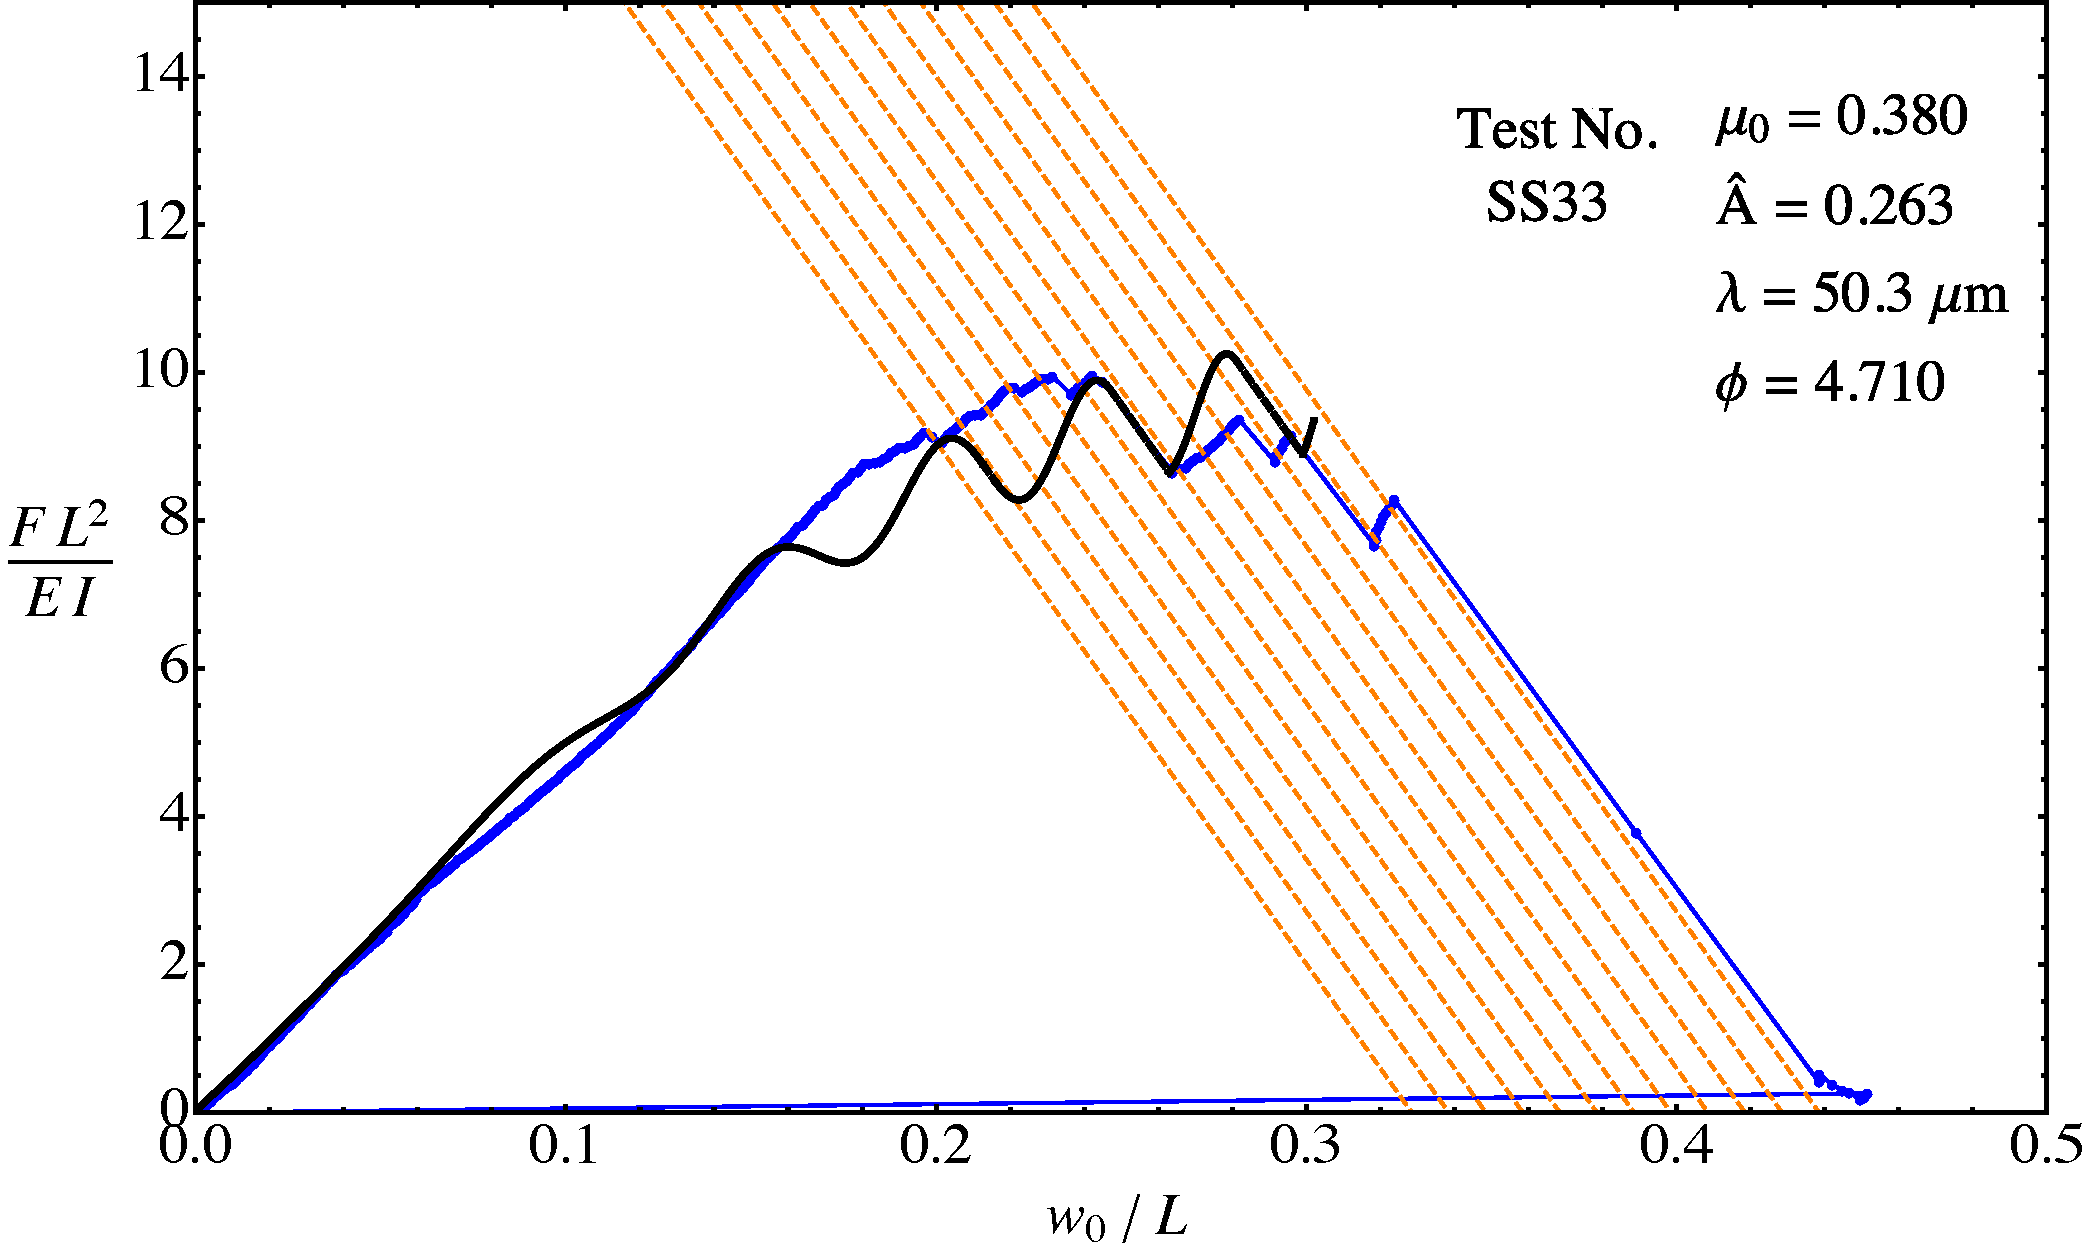
\includegraphics[width = .5\linewidth]{Figures/ComparisonThreeModels/Fitting20.pdf}}
\subfigure{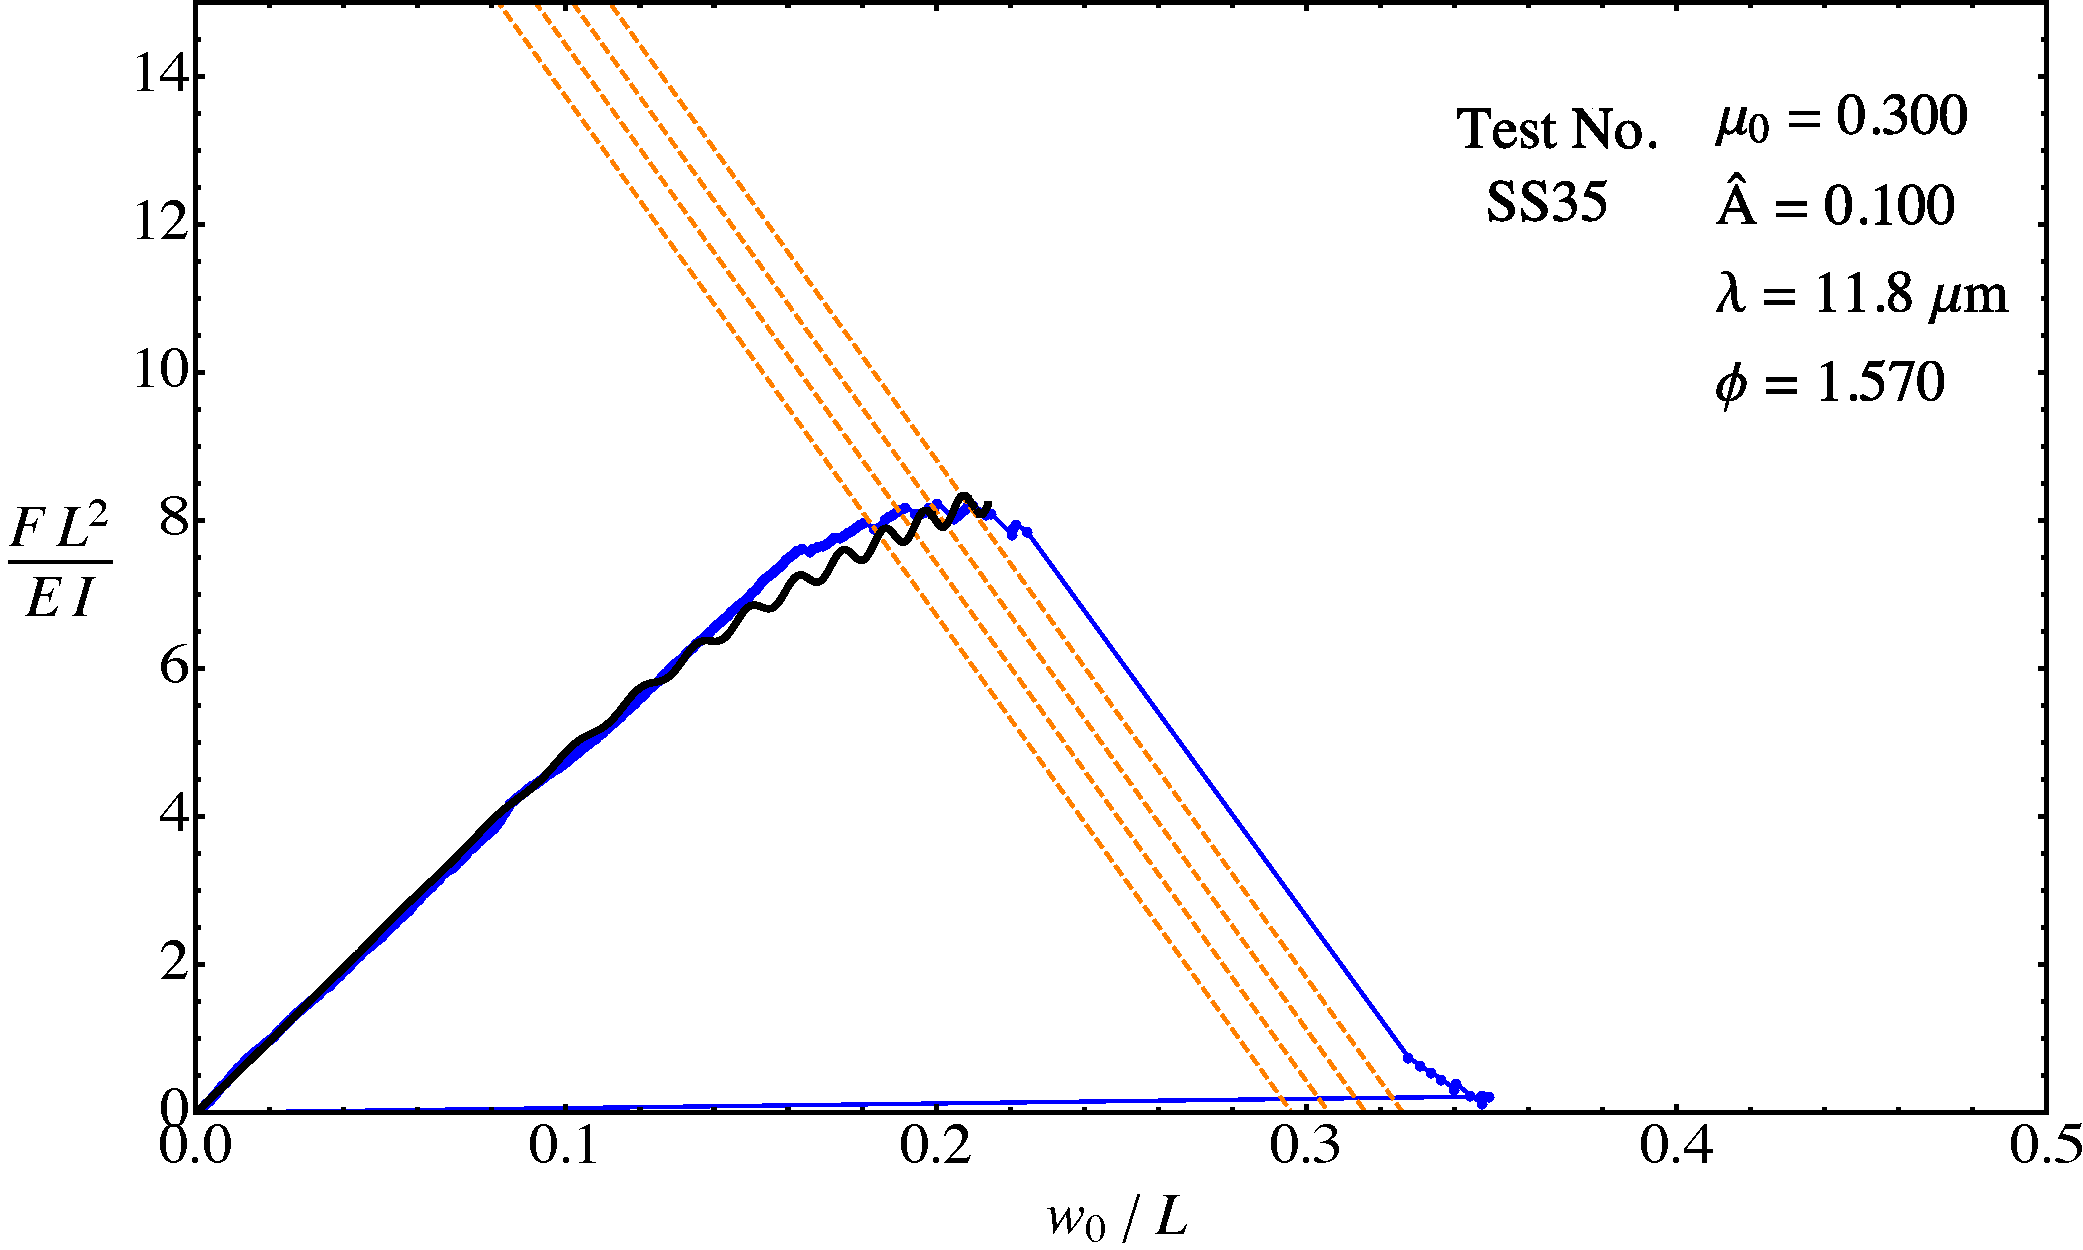
\includegraphics[width = .5\linewidth]{Figures/ComparisonThreeModels/Fitting21.pdf}}
\subfigure{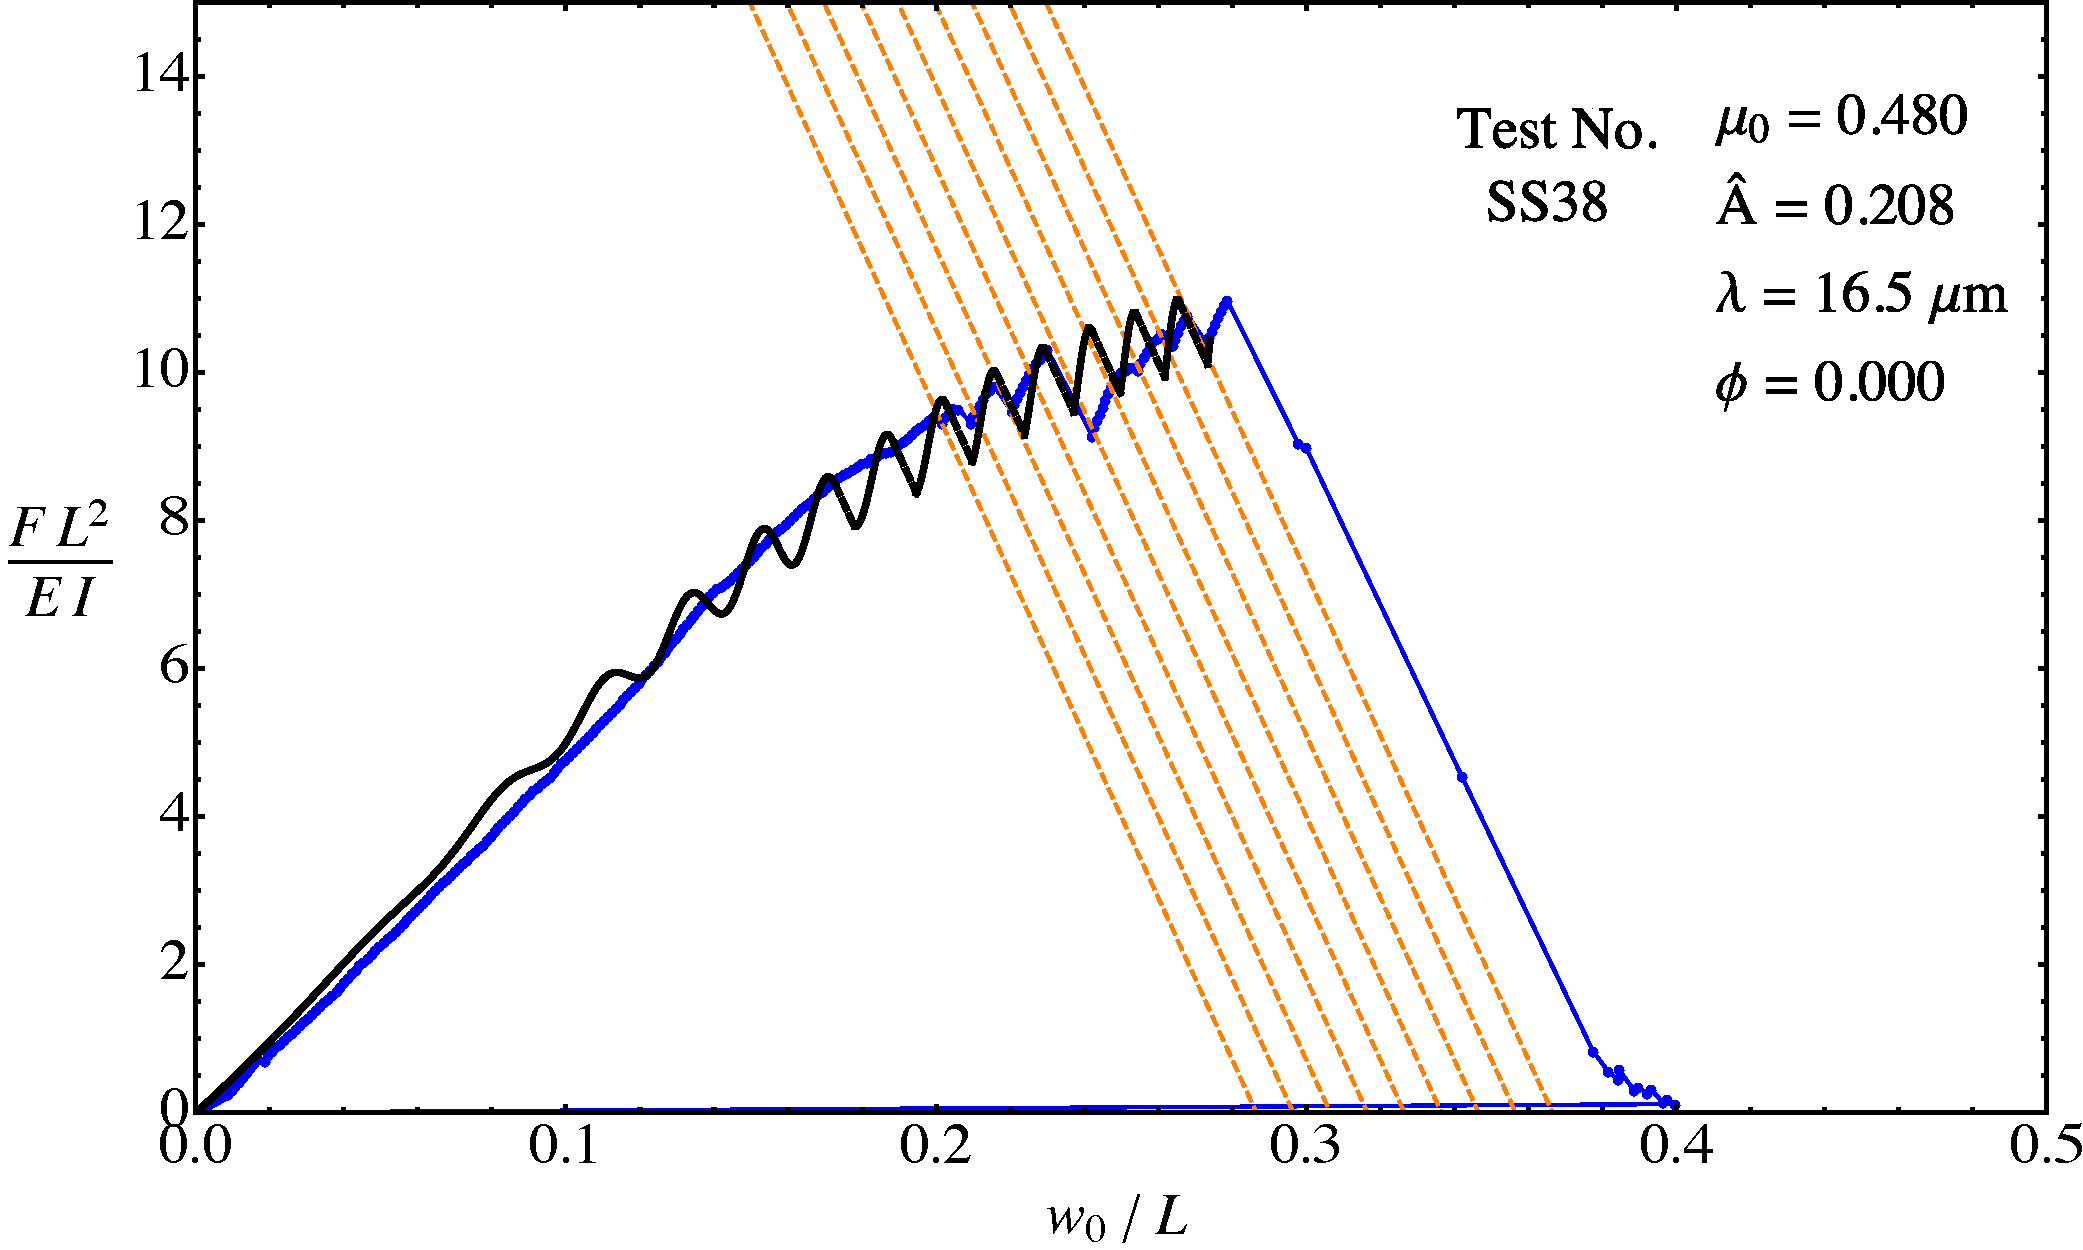
\includegraphics[width = .5\linewidth]{Figures/ComparisonThreeModels/Fitting22.pdf}}
\caption{Comparisons between the theoretical (black) and experimental (blue) $\hat{F}$-$\hat{w}_0$ response for simply-supported tests with sawtooth pattern (continued). The orange oblique lines describe the $\hat{F}$-$\hat{w}_0$ relations of the cantilever, the loading device in the test, as stage displacement $w_s$ increases.}
\end{figure}
%%%%%%%%%%%%%%% SS table 1




\clearpage
